\chapter{Ergebnisse}

In diesem Kapitel wird darauf eingegangen, welche Änderungen vorgenommen wurden, um den Algorithmus auf RGB-D Daten anwenden zu können. Es wird die verwendete RGB-D Kamera sowie die Hardware zur Gewinnung von Odometrieinformationen vorgestellt. Anschließend werden die Datensätze beschrieben, anhand derer der Algorithmus validiert wird. Für die Validierung muss der Algorithmus zunächst für die geänderte Sensorik und Umgebung parametrisiert werden. Um den Algorithmus für die geänderten Anwendungsbedingungen zu verbessern, wurde der Deskriptor neu trainiert. Die verwendeten Trainingsdaten sowie der Ablauf des Trainings werden erläutert und die Ergebnisse ausgewertet. Abschließend wird der Einfluss einer Erweiterung der Segmentierung, bei der Farbinformationen mit einbezogen werden, untersucht. 

\section{Setup}

Der SegMap-Algorithmus ist in das Robot Operating System (ROS) integriert. Dies ist ein Open Source Framework, das verschiedene Bibliotheken und Werkzeuge für die Entwicklung von Roboteranwendungen umfasst. Es bietet beispielsweise verschiedene Gerätetreiber und Visualisierungswerkzeuge sowie ein eigenes System zum Austausch von Nachrichten zwischen verschiedenen Prozessen.

%https://www.ros.org/

Um den Algorithmus für die Anwendung auf RGB-D Daten in einer indoor-Umgebung validieren zu können, werden indoor-Datensätze benötigt, die RGB-D Daten und Odometrieinformationen enthalten. Diese müssen in einer ROS-kompatiblen Form vorliegen. Hierfür wird der Nachrichten-Stream der verschiedenen Sensoren in von ROS definierten Sensornachrichtenformaten mit zugehörigem Zeitstempel in sogenannten Bag-Dateien gespeichert. 

Es gibt viele verschiedene frei verfügbare indoor RGB-D Datensätze, bei denen z.B. diverse Räume statisch mit einer RGB-D Kamera aufgenommen wurden. Die Daten müssen allerdings als Stream kontinuierlich aufeinander folgender Nachrichten in einem ROS-Sensornachrichtenformat zur Verfügung stehen. Es handelt sich um einen SLAM-Algorithmus bei dem die Trajektorie des Roboters sowie die entstehende Karte der Umgebung laufend durch die Erkennung von Loop Closures korrigiert werden. Daher muss der Datensatz für eine sinnvolle Validierung auch Schleifen enthalten, bei denen Teile der Umgebung mehrmals besucht werden. Eine Umwandlung der öffentlich zugänglichen Datensätze auf die genannten Anforderungen  ist sehr aufwendig. Daher wurde für die Validierung ein eigener Datensatz erstellt. 

Im Folgenden wird die verwendete Hardware für die Erstellung der Datensätze sowie die Ausstattung des für die Validierung des Algotihmus verwendeten Computers vorgestellt. Außerdem werden die Datensätze anhand derer die Validierung durchgeführt wird präsentiert und erläutert wie diese erstellt wurden.

\subsection[Kamera (Kopp)]{Kamera}
\label{sec:kamera}

Es gibt auf dem Markt viele verschiedene RGB-D Kameras. Diese unterscheiden sich typischerweise neben den Preisen, der Verfügbarkeit und ihrer physikalischen Dimensionen auch hinsichtlich des Blickwinkels, der Auflösung und der Reichweite. Außerdem werden Hersteller-abhängig unterschiedliche APIs geliefert, die sich hinsichtlich der Anwenderfreundlichkeit und der Hard- und Software-spezifischen Anforderungen zur Systemintegration unterscheiden. 

Für die Auswahl einer geeigneten Kamera für die Aufnahme der Datensätze wurden einige Kriterien aufgestellt, die von der Kamera erfüllt werden müssen. 

\subsubsection{Kriterien}

Da indoor-Umgebungen sich in der Regel nicht über große Entfernungen erstrecken, ist die Sichtweite recht beschränkt. Daher wird als relevanter Bereich für eine Orientierung in solchen Umgebungen ein Messbereich von bis zu 10 m Entfernung zum Sensor definiert. Die Reichweite der Kamera sollte etwa diese Entfernung abdecken. 

Der SegMap-Algorithmus ist auf die Verarbeitung der Daten eines hochauflösenden LiDAR-Sensors ausgelegt. Als relevanter Bereich für die Datenverarbeitung wurden 50 m gewählt. Die Validierung erfolgte anhand des KITTI-Odometrie Datensatzes. Zur Punktwolkenerzeugung wird dabei ein Velodyne HDL-64E Laserscanner verwendet. Um ähnlich gute Ergebnisse  zu erzielen, sollte die Kamera in der definierten maximalen Distanz von etwa 10 m über eine ähnlich gute Auflösung wie dieser, bezogen auf die geometrische Beschaffenheit der Umgebung, verfügen.

Die horizontale Auflösung des verwendeten Velodyne Scanners beträgt laut Datenblatt 0,08$^\circ$ die vertikale Auflösung 0.4$^\circ$. Wie bereits erwähnt, ist im Außenbereich eine Umgebung von bis zu 50 m Entfernung von Interesse. Um eine Vergleichbarkeit zu schaffen, muss die Auflösung auf die relevanten Entfernungen bezogen berechnet werden. Wie auf Abbildung \ref{fig:Auflösung} dargestellt, kann der Abstand $a_d$ zweier Punkte anhand der Entfernung $d$ zum Sensor und dem Winkel $\alpha$, der dem gegeben Winkel der Auflösung entspricht, berechnet werden. Hierfür wird folgende Formel verwendet:

\begin{align}
	a_d= d*sin(\alpha)/cos(\alpha)
\end{align}

Mit der gegebenen Auflösung und einer maximalen Entfernung von 50 m, ergibt sich somit ein horizontaler Punktabstand von $\sim$7 cm. In vertikaler Richtung beträgt der Punktabstand entsprechend $\sim$ 35 cm. Ein etwa 2$\times$2 m messende Fläche in 50 m Entfernung kann somit durch circa 140 Punkte repräsentiert werden. Damit wird es als Segment in die Karte geschrieben, da hierfür eine Begrenzung von mindestens 100 Punkten gesetzt ist. 

\begin{figure}
	\centering
	\includegraphics[width=0.5\linewidth]{Bilder/Aufloesung_Kamera_LIDAR.png}
	\caption{Darstellung der Auflösung anhand des Punktabstandes in einer definierten Entfernung d}
	\label{fig:Auflösung}
\end{figure}

Betrachtet man Strukturen, die im Innenbereich potentielle Segmente darstellen können, so stellen Türen, Tische, Schränke, Fenster oder auch ein hervorstehender Lichtschalter potentielle Kandidaten dar. Daraus abgeleitet ergibt sich das Kriterium Strukturen mit Kantenlängen ab 10$\times$10 cm in einer Entfernung ab 50 cm genügend Punkte für eine Segmentierung zuordnen zu können. Auf eine Entfernung von 10 m sollten Türen und Schränke noch sicher Segmente ergeben. 

Zusätzlich sollte es für die Kamera eine ROS-Anbindung geben, um eine einfache Generierung der Daten im benötigten ROS-Sensornachrichtenformat zu ermöglichen. Außerdem sollte eine Framerate von 10 Hz erreicht werden und die Kamera einfach auf dem Markt verfügbar sein. 

%Da der SegMap-Algorithmus mit LiDAR Daten arbeitet, erfolgt eine Gegenüberstellung der erreichten Auflösung der jeweiligen Systeme. Dabei ist zu berücksichtigen in welcher Entfernung die jeweiligen Sensoren relevante Informationen aufnehmen. Im Außenbereich beträgt dieser relevante Bereich zwischen 3 m und 50 m Entfernung. Für den Innenbereich wird definiert, dass zwischen 0,5 m und 10 m der relevante Messbereich liegt. Die Auflösung im Innenbereich sollte in der formulierten Distanz ausreichend hoch gewählt werden, um Segmente anhand der geometrischen Beschaffenheit der Umgebung zu erzeugen.

%Die Verfasser des SegMap Algorithmus verwenden in ihren Experimenten den KITTI Odometrie Datensatz. Zur Punktwolkenerzeugung wird dabei ein Velodyne HDL-64E Laserscanner verwendet. Die Auflösungen der jeweiligen Sensoren müssen einmal in horizontaler und einmal in vertikaler Auflösung verglichen werden. Die horizontale Auflösung des Velodyne Scanners beträgt laut Datenblatt $0,08^\circ$ die vertikale Auflösung $0.4^\circ$. Wie bereits erwähnt, ist im Außenbereich eine Umgebung von 3-50 m von Interesse. Um eine Vergleichbarkeit zu schaffen, muss die Auflösung auf die relevanten Entfernungen bezogen berechnet werden. $a_d$ steht dabei für den Abstand zweier Punkte in einer Entfernung $d$, siehe Abbildung \ref{fig:Auflösung}. Mit dem gegebenen Winkel $\alpha$ und einer Entfernung von 50 m ergibt sich mit $ a_d= d*sin(\alpha)/cos(\alpha)$ ein Punktabstand von $\backsim$ 7 cm bei $d$ = 10m von $\backsim$ 1,4cm. Die horizontale Auflösung in 10 Metern beträgt $\backsim$ 7 cm, in 50m Entfernung $\backsim$ 35cm. Ein etwa $2 \times 2$m  messendes Objekt in 10 m Entfernung kann somit durch ca. 4000 Punkte repräsentiert werden.  In einer Entfernung von 50 m erzeugt die gleiche Fläche ca. 140 Punkte. Ein Segment wird ab einer Mindestpunktzahl von 100 Punkten als solches verarbeitet, die maximale Punktzahl beträgt 15000 Punkte. Betrachtet man Strukturen die im Innenbereich potentielle Segmente darstellen können, so stellen Türen, Tische, Schränke, Fenster oder auch ein hervorstehender Lichtschalter potentielle Kandidaten dar. Daraus abgeleitet entstand das Kriterium Strukturen mit Kantenlängen ab $10\times 10$cm in einer Entfernung ab 50 cm genügend Punkte für eine Segmentierung zuordenen zu können. Auf eine Entfernung von 10 m sollten Türen und Fenster noch sicher Segmente ergeben. Die auf dem Markt erhältlichen Kameramodelle, die in der folgenden Tabelle aufgeführt sind, werden auf deren Auflösung, Preis, Framerate, Verfügbarkeit, Baugröße, Bildausschnitt und Typ  hin geprüft.


\subsubsection{Intel Realsense D435}

In Tabelle \ref{tab:Kameras} sind die technischen Eigenschaften einiger auf dem Markt erhältlichen Kameramodelle aufgeführt. Sie verfügen alle über eine ROS-Anbindung und liefern zusätzlich zu den Tiefeninformationen ein Farbbild. Hinsichtlich der genannten Kriterien werden die verschiedenen Kameras geprüft, ob diese erfüllt werden. Außerdem werden die Preise sowie die Baugröße verglichen. In der Tabelle beschreibt FOV das Sichtfeld, das in horizontaler und vertikaler Richtung abgedeckt wird. 

%Die auf dem Markt erhältlichen Kameramodelle, die in der folgenden Tabelle aufgeführt sind, werden auf deren Auflösung, Preis, Framerate, Verfügbarkeit, Baugröße, Bildausschnitt und Typ  hin geprüft.

\begin {table}[th!]
\setlength{\tabcolsep}{0.6mm}
\begin{tiny}
 \centering
 \caption{Technische Daten verschiedener RGB-D Kameras mit Ros-Anbindung}
 \label{tab:Kameras}
 \begin{tabulary}{\textwidth}{ L C C C C C C C C }
  \hhline{=========}
    Kamera & Typ & Reichweite (m) & 3D-Auflösung & RGB-Auflösung & Framerrate (fps) & FOV & Abmessungen (mm) & Preis (Euro)\\
  \hhline{=========}
  Microsoft® Kinect™ 2.0 & Time of flight & 0.5-4.5 & 512$\times$424 & 192$\times$1080 & 30 & 70$^\circ$H, 60$^\circ$V & 250$\times$70$\times$45 & 149  \\
  \hhline{---------}
  ASUS® XtionPro™ Live & Structured Light &  0.8-3.5 & 640$\times$480 & 1280$\times$1024 & 30 & 58$^\circ$H, 45$^\circ$V & 180$\times$40$\times$25 & - \\
  \hhline{---------}
  Stereolabs® ZED™& Embedded Stereo & 1.5-20 & 2208$\times$1242 & 2208$\times$1242 & 15-120 & 96$^\circ$H, 54$^\circ$V & 175$\times$30$\times$33 & 349 \\
  \hhline{---------}
  CarnegieRobotics® MultiSense™ S7 & Embedded Stereo & 0.4m-$\infty$ & 2048$\times$1088 & 2048$\times$1088 & 15 & 80$^\circ$H, 45$^\circ$V & 130$\times$130$\times$65 & - \\
  \hhline{---------}
  Ensenso® N35-606-16-BL & Structured Light & - & 1280$\times$1024 & 1280$\times$1024 & 10 & 58$^\circ$H, 52$^\circ$V & 175$\times$50$\times$52 & - \\
  \hhline{---------}
  Nerian SceneScan & FPGA Stereo Camera & - & 1856$\times$1856 & 1856$\times$1856 & 100 & - & 144$\times$41$\times$35mm & - \\
  \hhline{---------}
  Intel® RealSense™ Camera D415 & Active IR Stereo & 0.3-10 & 1280$\times$720 & 1920$\times$1080 & 30-90 & 63.4$^\circ$H, 40.4$^\circ$V & 99$\times$20$\times$23 & 167 \\
  \hhline{---------}
  Intel® RealSense™ Camera D435 & Active IR Stereo & 0.105-10 & 1280$\times$720 & 1920$\times$1080 & 30-90 & 85.2$^\circ$H, 58$^\circ$V & 99$\times$25$\times$25 & 200 \\
  \hhline{---------}
  FRAMOS Depth Camera D435e & Active IR Stereo & 0.2-10 & 1280$\times$720 & 1920$\times$1080 & 30 & 86$^\circ$H, 57$^\circ$V & - & - \\
  \hhline{---------}
  Orbbec® Astra Mini™ & Structured Light & 0.6-5 & 640$\times$480 & 640$\times$480 & 30 & 60$^\circ$H, 49.5$^\circ$V & 80$\times$20$\times$20 & 185 \\
  \hhline{---------}
  Arcure Omega & Stereo & 0.3-50 & 1280$\times$1024 & 1280$\times$1024 & 60 & 120$^\circ$H, 90$^\circ$V & 200$\times$83$\times$79 & - \\
   \hhline{=========}
\end{tabulary}
\end{tiny}
\end{table}
%
%\begin{table}
%\label{tab:Kameras}
%	\caption{Technische Daten verschiedener RGB-D Kameras mit Ros-Anbindung}
%\begin{flushleft}
%\begin{tiny}
%\setlength{\tabcolsep}{0.6mm}
%\begin{tabular}[h]{@{}p{3cm}|p{1,5cm}|c|c|c|c|c|c|c|}
%Kamera&Typ&Reichweite&3D Auflösung&RGB Auflösung&Framerrate&FOV & Abmessungen &  Preis \\
%\hline
%Microsoft® Kinect™ 2.0 & Time of flight&0.5-4.5m&512x424&1920x1080&30fps&70$^\circ$H,60$^\circ$V&250x70x45mm&149  \\
%\hline
%ASUS® XtionPro™ Live & Structured light&0.8-3.5m&640x480&1280x1024&30fps&58$^\circ$H,45$^\circ$V& 180x40x25mm&-  \\
%\hline
%Stereolabs® ZED™& Embedded stereo&1.5-20m&2208x1242&2208x1242&15-120 fps&96$^\circ$H,54$^\circ$V& 175x30x33mm& 349 \\
%\hline
%CarnegieRobotics® MultiSense™ S7&Embedded stereo&0.4m-$\infty$ &2048x1088&2048x1088&15 fps&80$^\circ$H,45$^\circ$V&130x130x65 mm & -  \\
%\hline
%Ensenso® N35-606-16-BL & Structured light&-&1280x1024&1280x1024&10fps&58$^\circ$H,52$^\circ$V&175x50x52mm&- \\
%\hline
%Nerian SceneScan&FPGA Stereo Camera&-&1856x1856&1856x1856&100fps&-&144x41x35mm&-  \\
%\hline
%Intel® RealSense™ Camera D415&Active IR Stereo&0.3-10m&1280x720&1920x1080&30-90fps&63.4$^\circ$H,40.4$^\circ$V&99x20x23mm&167  \\
% \hline
%Intel® RealSense™ Camera D435&Active IR Stereo&0.105-10m&1280x720&1920x1080&30-90fps&85.2$^\circ$H,58$^\circ$V& 99x25x25mm&200  \\
% \hline
%FRAMOS Depth Camera D435e&Active IR Stereo&0.2-10m&1280x720&1920x1080&30fps&86$^\circ$H,57$^\circ$V&-&-  \\
% \hline
%Orbbec® Astra Mini™&Structured Light &0.6-5m&640x480&640x480&30fps&60$^\circ$H,49.5$^\circ$V &80x20x20mm&185  \\
% \hline
%Arcure Omega& Stereo&0.3-50m&1280x1024&1280x1024&60fps&120$^\circ$H,90$^\circ$V&200x83x79mm& -  \\
%\end{tabular}
%\end{tiny}
%\end{flushleft}
%\end{table}

Aufgrund des hohen Blickwinkels, der kompakten Bauweise, der schnellen Verfügbarkeit und des niedrigen Preises wird von allen Kameras, die die genannten Kriterien erfüllen, die Realsense D435 der Firma Intel gewählt. Diese nutzt für die Generierung der Punktwolke den Ansatz der aktiven Stereoskopie. Die Auflösung der Punktwolke liegt bei maximal 1280x720 Punkten. Werden nun die gleichen Überlegungen angestellt, wie bei der Analyse des LiDAR-Sensors, ergeben sich bei einer Distanz von 10 m eine horizontale Auflösung von $\sim$15,1 mm und eine vertikale Auflösung von $\sim$14,6 mm. Entsprechend ergeben sich bei einer Entfernung von 0,5 m ein Punktabstand von 0,73 mm in horizontaler und 0,75 mm in vertikaler Richtung. 

Die zuvor angedachte Fläche von 10x10cm in einer Entfernung von 50cm liefern also $\sim$137$\times$133 $\approx$ 23000 Messpunkte. In einer Entfernung von 10 m stehen für eine Fläche von 200x100cm dementsprechend 143$\times$67 $\approx$ 9438 Messpunkte zur Verfügung. Daraus ergibt sich, dass die Auflösung der Kamera hoch genug ist, um typische indoor-Objekte mit der geforderten Punktdichte abzutasten. 

%kommt man bei einer Distanz von 50cm auf eine vertikale Auflösung von $\sim$ 0,73 mm und eine horizontale Auflösung von $\sim$ 0,75mm. Bei einer Entfernung von 10 m beträgt die vertikale Auflösung $\sim$ 14,6 mm, die horizontale Auflösung beträgt $\sim$ 15,1 mm. Die zuvor angedachten 10x10cm in einer Entfernung von 50cm liefern also  $\sim$ 137x133$\approx$ 23000 Messpunkte. In einer Entfernung von 10 m stehen für eine Struktur von 200x100cm dementsprechend 143x67$\approx$9438 Messpunkte zur Verfügung. Aufgrund dieser Berechnung, des günstigen Preises, der kleinen Abmessungen und des geringen Gewichts, aber auch die einfache Integrierung in das ROS Framework, durch bestehende Libraries wurde entschieden diese Kamera zu beziehen.

\subsubsection{Erweiterung des Sichtfelds} 
\label{sec:stereo}
 
Im vorherigen Abschnitt wurde erläutert, dass die Punktwolke, die die gewählte RGB-D Kamera erzeugt, ausreichend auflösend ist. Der horizontale Blickwinkel des bei SegMap verwendeten Laserscanners beträgt 360$^\circ$, der Blickwinkel der Kamera jedoch lediglich 85,2$^\circ$. Daher wurde die Überlegung angestellt den Öffnungswinkel zu verbreitern, um die Umgebung besser einfangen zu können. 

Angedacht war die Kamera aktiv durch einen Motor rotieren zu lassen. Die Abbildung \ref{fig:Dreheinheit} zeigt die dafür konstruierte Rotationseinheit. Der horizontale Aufnahmewinkel wird dadurch auf 198$^\circ$ erweitert. Für langsame Bewegungen eines Roboters kann das ein guter Ansatz sein. Bei höherer Geschwindigkeit ist die Gefahr groß Verarbeitungsfehler zu bekommen, da die Bewegungen der Kamera abhängig von der Bewegung der Plattform im Raum sehr genau bestimmt werden muss, um eine konsistente Punktwolke zu generieren.

Eine Alternative stellt eine fixierte Anordnungen von zwei Kameras, wie in Abbildung \ref{fig:Kamera_Starr} zu sehen, dar. Der Winkel zwischen den Kameras wurde so gewählt, dass sich die Punktwolken ab einer Entfernung von 30 cm überlappen. Der Sichtbereich vergrößert sich so auf 158$^\circ$. Die Verarbeitung der Punktwolken durch den fixierten Abstand und Winkel ist sehr viel einfacher als bei einer schwenkbaren Lösung und weniger Fehleranfällig. Anordnungen mit mehr als zwei Kameras wurden nicht in Betracht gezogen, da so der Kostenvorteil gegenüber eines 360$^\circ$ Laser verloren gehen würde. Auch ist die Verarbeitung von mehr als zwei Punktwolken auf kleineren Rechnersystemen schwer umsetzbar.

\begin{figure}
	\centering
	\begin {minipage}[t]{0.45\linewidth}
	\centering
	\includegraphics[width=\linewidth]{Bilder/Kameradreheinheit1.png}
	\caption{Darstellung der motorbetriebenen Dreheinheit mit Kamera}
	\label{fig:Dreheinheit}
	\label{fig:Kamera_Starr}
\end{minipage}
\hfill
 \begin{minipage}[t]{0.45\linewidth}
	\centering
	\includegraphics[width=\linewidth]{Bilder/Kamera_Starr.png}
	\caption{Darstellung der starren Anordnung zweier Kameras}
	\label{fig:Kamera_Starr}
\end{minipage}
\end{figure}

\subsection[Odometrie (Kopp)]{Odometrie}

Der SegMap-Algorithmus benötigt Odometrieinformationen. Die Erzeugung von Odometriedaten einer Roboterplattform kann Hardwareseitig beispielsweise durch Drehgeber an den Achsen oder anhand der Steuerbefehlen geschehen. Außerdem kann Software-basiert, etwa über ICP eine Odometrieschätzung erzeugt werden. Beim SegMap-Algorithmus kann die Trajektorie sowohl anhand Hardware-basierter Odometrieinformtionen als auch durch ICP geschätzt werden. Zusätzlich können beide Verfahren auch fusioniert werden. Jedoch wurde der mitgelieferte ICP-Algorithmus für outdoor-Umgebungen und 360$^\circ$ Rundumsicht parametrisiert. Die Parametrierung hat gezeigt, dass keine guten Ergebnisse für die untersuchten Anwendungsszenarien erzielt werden. 

Auf Abbildung \ref{fig:ICP} sind Beispiele für die Trajektorie dargestellt, die der SegMap-Algorithmus ermittelt. In (a) ist die Trajektorie zu sehen, die sich aus den Odoemtrieinformationen ergeben, die mit der verwendeten Vorrichtung ermittelt wurden. Diese wird im weiteren Verlauf dieses Kapitels beschrieben. In (b) ist die Trajektorie des gleichen Datensatzes dargestellt, die durch eine Fusionierung der selben Odometrieinformationen wie in (a) mit dem mitgelieferten ICP Algorithmus ermittelt wird. Die Trajektorie wird durch die Fusionierung mit ICP deutlich verschoben. In (c) ist dieselbe Trajektorie aus einem Blickpunkt in der x,z-Ebene dargestellt. Dies zeigt, dass die Trajektorie auch in z-Richtung verschoben wird, obwohl der Datensatz auf einer Ebene ohne Änderungen der z-Koordinaten aufgenommen wurde. Daher wird der mitgelieferte ICP-Algorithmus nicht verwendet. ICP eignet sich besser für die Zuordnung von 360$^\circ$ Punktwolken, da durch die höhere Punktmenge mehr Korrespondenzen gefunden werden können. Dadurch werden zuverlässigere Ergebnisse geliefert.

\begin{figure}
	\centering
	\includegraphics[width=\linewidth]{Bilder/bb_icp_zusammen.png}
	\caption{Beispiele für die erzeugten Trajektorie anhand (a) der Odometrieinformation sowie (b) und (c) nur durch ICP}
	\label{fig:ICP}
\end{figure}

Eine verbreitete Anwendung zur Erzeugung von Odometrieinformationen anhand von Bildern oder Punktwolken für ROS stellt RTAB-Map dar. Dies ist ein Graphen-basierter SLAM-Ansatz, der sowohl auf RGB-D und Stereo Daten als auch auf LiDAR Daten angewendet werden kann. Dieser liefert eine ICP-basierte Trajektorienschätzung und kann einfach durch einen ROS-Wrapper eingebunden werden. In mehreren Messfahrten lieferte RTAB-Map jedoch keine zufriedenstellenden Ergebnisse mit der genutzten Hardware. Um das Augenmerk auf die Verbesserung des SegMap-Algorithmus zu lenken, wurde daher eine Hardware-basierte Odometrie für die Erzeugung der Datensätzen verwendet. 

Hierfür wurde eine einfache Plattform gebaut, die auf Rädern durch die Umgebung geschoben werden kann. Die Räder sind wie bei einem Differentialantrieb angeordnet. Hierbei befinden sich zwei Räder auf einer Achse, die sich unabhängig voneinander drehen. Die Plattform wird durch ein Stützrad stabilisiert. Abbildung \ref{fig:Differentialantrieb} verdeutlicht das Prinzip, wie bei einem Differentialantrieb die Bewegung des Roboters ermittelt wird. Diese ergibt sich aus dem Unterschied der Geschwindigkeit mit der sich die Räder drehen. 

\begin{figure}
	\centering
	\includegraphics[width=\linewidth]{Bilder/Roboter_Differenzial_antrieb.png}
	\caption{Darstellung des Prinzips eines Differentialantriebs}
	\label{fig:Differentialantrieb}
\end{figure}

In Abbildung \ref{fig:Laboter} ist die Vorrichtung zur Erzeugung der Datensätze zu sehen. Hierbei wird die Kamera in einer Höhe von 0,85 cm über dem Boden auf die Plattform montiert.

\begin{figure}
	\centering
	\begin {minipage}[t]{0.3\linewidth}
	\centering
	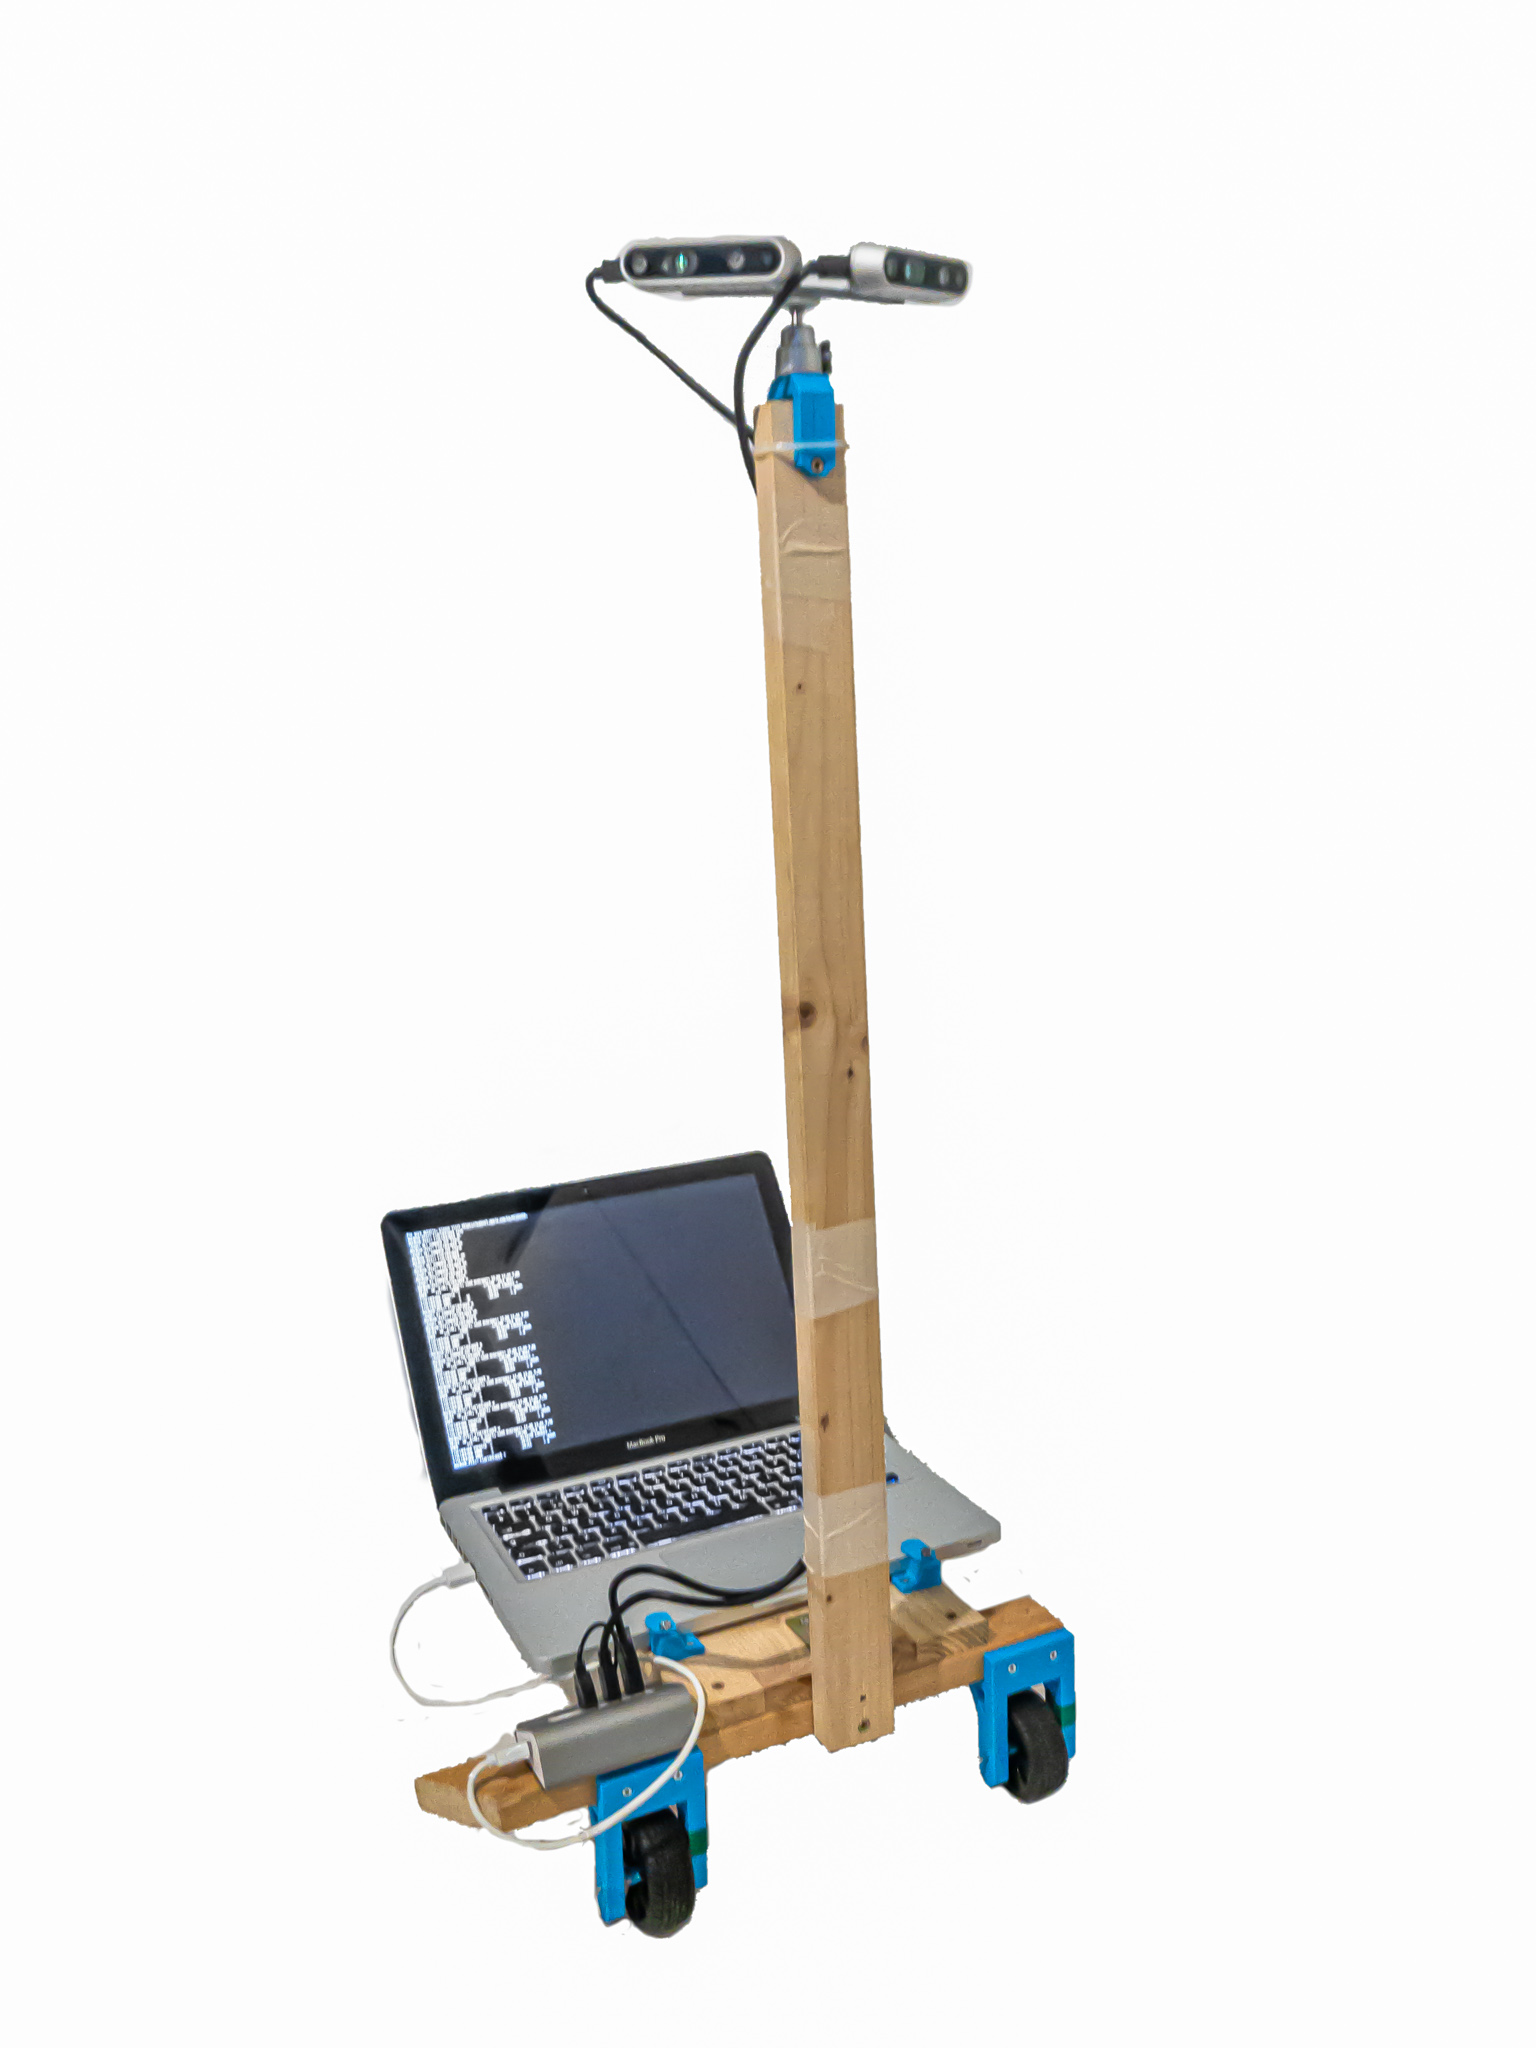
\includegraphics[width=\linewidth]{Bilder/laboter.png}
	\caption{Plattform für Datenaufzeichnung }
	\label{fig:Laboter}
\end{minipage}
\hfill
 \begin{minipage}[t]{0.6\linewidth}
	\centering
	\includegraphics[width=\linewidth]{Bilder/Roboter_Differenzial_antrieb_2.png}
	\caption{Darstellung des Prinzips zur Ermittlung der neuen Pose }
	\label{fig:Odoemtrie}
\end{minipage}
\end{figure}

Die kostengünstigste und einfachste Lösung zur Erfassung von Odometrieinformationen stellen Drehgeber an den Rädern dar. Hierbei sind die Räder in 20 gleich große Kreisabschnitte aufgeteilt. Die Drehgeber erfassen, wie viele dieser Kreisabschnitte pro Rad durch die Rotation durchlaufen wurden. Aus der Anzahl der passierten Kreisabschnitte und dem Raddurchmesser kann die zurückgelegte Distanz eines Rads ermittelt werden. Hierbei sind nur die beiden Räder, die auf einer Achse liegen, mit Drehgebern ausgestattet, am Stützrad erfolgt keine Messung. Aus dem Abstand zwischen den beiden Rädern und den zurückgelegten Strecken pro Rad und pro Zeitschritt kann die Bewegung des Roboters ermittelt werden. Dies ist auf Abbildung \ref{fig:Odoemtrie} dargestellt. Die neue Posenschätzung ergibt sich durch folgende Gleichungen: 

\begin{subequations}
	\begin{align}
		\theta &= \theta + \dfrac{s_R-s_L}{l} \\
		x &= x + \dfrac{s_R+s_L}{2}*cos(\theta) \\
		y &= y + \dfrac{s_R+s_L}{2}*sin(\theta)
	\end{align}
\end{subequations}

Die Posenschätzungen werden mit einer Frequenz von 10 Hz ermittelt. Bei dieser Varinte der Odometriesschätzung werden nur x,y,$\theta$-Posen geschätzt. Diese beschreiben die lage im raum in x,y-Richtung sowie den Winkel um die z-Achse. Da die Datensätze nur in Umgebungen auf ebenen Flächen aufgezeichnet wurden, ist diese Posenerfassung ausreichend.

Die Verarbeitung der Pulse, die die Inkrementalgeber erzeugen, übernimmt ein Arduino nano Mikrocontrollerboard auf Basis der ATmega328 MPU. Die Odometrieinformationen in Form von x,y,$\theta$-Posen werden auf dem Arduino berechnet und im ROS-Nachrichtenformat tf2/TFMessage gepuplished. Die Verbindung zum Rechner erfolgt über USB mit dem ROS-Bibliothek rosserial$\_$arduino. 

Die Genauigkeit der erzeugten Odometrieinformation wurde überprüft, indem eine zuvor ausgemessene Strecke von 41,5 m ($\pm$4,1mm Maßbandabweichung) in Form eines U abgefahren wurde. Diese ist auf Abbildung \ref{fig:Test_Odometrie} dargestellt. Der Versuch wurde zehn Mal durchgeführt. Die aufgezeichnete Strecken wiesen dabei in x-Richtung eine Streuung von 15\% auf. In y-Richtung betrugen die Streuungen 7\%. Die gesamt zurückgelegte Strecke variierte im Bereich von $\pm$60 cm. Diese Genauigkeit wurde als ausreichend für den angestrebten nutzen bewertet.

\begin{figure}
	\centering
	\includegraphics[width=0.75\linewidth]{Bilder/Test_odometrie.png}
	\caption{Test Genauigkeit der Odometrieinformationen}
	\label{fig:Test_Odometrie}
\end{figure}

\subsection{Ausstattung des Computers}

Für die Validierung des SegMap-Algorithmus wird eine Intel i7-7700 @ 3,6 GHz CPU sowie eine Nvidia Quadro P2000 GPU mit 5 GB Speicher verwendet. Außerdem stehen 16 GB DDR4 RAM zur Verfügung. Verwendet wurde das Betriebssystem Ubuntu 16.04 und die ROS-Version kinetic. Für das künstliche neuronale Netz wurde Tensorflow 1.8 genutzt. 

\subsection[Datensätze (Schmelzer)]{Datensätze}
\label{sec:Datensatz}

Zur Validierung des SegMap-Algorithmus werden indoor-Datensätze benötigt, die mit einer RGB-D Kamera erzeugt wurden. Außerdem werden Odometrieinformationen benötigt über die die ungefähre Pose des Roboters geschätzt werden kann. Die bereits erwähnten Anforderungen werden lediglich von SLAM-Datensätzen der TU München erfüllt. Daher wurden zusätzlich eigene Datensätze erstellt, um die Ergebnisse der Anwendung des Algorithmus umfassender analysieren zu können. Außerdem müssen ausreichend Trainingsdaten für das Training des Deskriptors erzeugt werden. 

Die verschiedenen Sensordaten werden in unterschiedlichen ROS-Sensornachrichtenformaten erwartet, die eine spezifische Datenstruktur vorgeben. Diese müssen auf teilweise vorgegebenen Topics gepublisht werden. In ROS stellen Topics Busse dar, über die verschiedene Programmknoten Nachrichten austauschen. Hierbei ist jedoch fest definiert, welche Knoten senden und welche empfangen. Alle Nachrichten werden vom Algorithmus mit einer Rate von 10 Hz erwartet. 

Der Algorithmus lauscht auf vier verschiedene Nachrichten. Diese umfassen zum einen die Tiefeninformationen der Umgebungsabtastung im  sensor$\_$msgs/PointCloud2-Nachrichtenformat. Außerdem werden die Odometrieinformationen als Posenschätzung mit Zeitstempel in Form von geometry$\_$msgs/PoseStamped erwartet. Diese werden im Koordinatensystem der Roboterplattform angegeben, das sich mit dieser durch den Raum bewegt. Die Posenschätzung ist relativ zum Startpunkt des  Roboters, der den Ursprung des Odometrie-Koordinatensystems bildet. Daher wird zusätzlich zu jeder Posenschätzung die zugehörige Transformation vom Odometrie-Koordinatensystem zum Koordinanensystem der Roboterplattform mit demselben Zeitstempel benötigt, um eine Posenschätzung relativ zum Startpunkt des Roboters zu erhalten. Diese wird als Nachricht der Form geometry$\_$msgs/TransformStamped erwartet. Darüber hinaus werden alle Transformationen vom Odometrie-Koordinatensystem des Startpunkts der Odometrieaufzeichnungen bis zum Koordinanensystem der Kamera als tf2$\_$msgs/TFMessage benötigt. Tf2 ist eine ROS-Bibliothek für die Handhabung mehrere Transformationen. Es werden alle Beziehungen zwischen den Koordinatensystemen verfolgt und in einem Buffer gespeichert. Alle Transformationen werden im /tf Topic gepublisht. 

Die Datensätze wurden alle in Form von bag-Dateien gespeichert. Dies ist ein Dateiformat, in dem seriell ROS-Nachrichten in der Reihenfolge gespeichert werden, in der sie empfangen werden. Bei der Aufzeichnung wird für jedes Topic, dessen Nachrichten gespeichert werden sollen, ein Subscriber gestartet, der auf diese Nachrichten lauscht. Anschließend können die gespeicherten Nachrichten abgespielt werden, indem diese durch einen Publisher für andere Programmknoten veröffentlicht werden. Dadurch können die Sensornachrichten in ihrer genauen Zeitlichen Abfolge gespeichert werden und erscheinen dem Algorithmus beim abspielen, wie wenn die Nachrichten gerade von den Sensoren erzeugt wurden. 

\subsubsection{TUM Datensatz}
%https://vision.in.tum.de/data/datasets/rgbd-dataset

Die TU München stellt eine Sammlung von RGB-D Datensätzen für die Evaluierung visueller Odometrie und SLAM-Algorithmen frei zur Verfügung. Verwendet wurden Datensätze der Kategorie Robot SLAM, die zusätzlich zu den RGB-D Daten auch Odometrieinformationen enthalten. Diese Datensätze wurden erstellt, indem eine Microsoft Kinect auf einem Pioneer Roboter montiert wurde. Dies ist eine kleine Roboterplattform, die in diesem Fall ferngesteuert wurde und die Odometriedaten aufgezeichnet hat. 

Die Tiefenbilder, die von der Microsoft Kinect erzeugt werden, haben eine Auflösung von 640$\times$480 Pixeln und werden mit einer Framerate von 30 Hz geliefert. Die Kamera verfügt über eine Reichweite von 4,5 m.

Die Datensätze wurden in einer Halle aufgezeichnet, in der durch verschiedene Objekte eine Umgebung aufgebaut wurde. Es wurden beispielsweise mehrere Trennwände aufgestellt und verschiedene andere Objekte um diese herum arrangiert, wie Stühle, Stative und ein Teddybär. 

So wurden drei verschiedene Datensätze aufgezeichnet, bei denen der Pioneer unterschiedlich durch die Umgebung navigiert wurde. Die Datensätze enthalten Schleifen, bei denen Teile des Roboterpfads mehrmals abgefahren wurden. 

Die Datensätzen können direkt in Form eines Bag-Files heruntergeladen werden. Da diese jedoch mit einer älteren ROS-Version aufgenommen wurden, mussten diese zunächst in das Formt der verwendeten ROS-Version migriert werden. Hierfür werden von ROS bereits Funktionen mitgeliefert, die dies umsetzen. Außerdem werden die Nachrichten mit einer viel zu hohen Framerate gepublisht. Daher werden alle auf 10 Hz heruntergesetzt. Die Tiefeninformationen liegen im Bag-File lediglich in Form eines Tiefenbildes im Nachrichtenformat sensor$\_$msgs/Image vor.Diese Nachrichten wurden mithilfe des mit ROS mitgelieferten depth$\_$image$\_$proc Nodes in eine Punktwolke umgewandelt. 

Die Odometrieinformtionen sind in den Transformationsnachrichten des Topics /tf enthalten. Diese werden von der ersten Transformation vom ortsfesten Odometrie-Koordinatnesystem zum Koordinatensystem der Roboterplattform gebildet. Um diese Nachrichten in die vom Algorithmus erwartete Form zu überführe, wird ein Subscriber erstellt, der auf die Transformationsnachrichten lauscht. Anschließend werden die Informationen dieser Nachrichten in die benötigten Formate geometry$\_$msgs/PoseStamped und geometry$\_$msgs/TransformStamped umgewandelt und erneut in zwei neuen Topics gepublisht. 

Wie bereits erwähnt, müssen alle Transformationen vom Odometrie-Koordinatnesystem bis zum Kamera-Koordinatensystem, in dem die Tifeninformationen aufgenommen wurden, im /tf Topic gepublisht werden. Die Nachrichten sollten den gleichen Zeitstempel haben damit keine  Time-out Fehler bei der Verarbeitung der Informationen im Algorithmus auftreten. Daher wird ebenfalls der bereits erwähnte Subscriber auf die Transformation vom Odometrie-Koordinatensystem auf das Koordinatensystem der Roboterplattform verwendet. Sobald die Transformation empfangen wird, werden aus dem Transformationsbuffer die aktuellsten Transformationen zwischen den übrigen Koordinatensystemen bis zum kamerakoordinatensystem gelesen. Alle Transformationen werden gemeinsam  mit einer Rate von 10 Hz gepublisht. 

\begin{figure}
	\centering
	\includegraphics[width=\linewidth]{Bilder/TUM_Manipulation.png}
	\caption{Darstellung der Vorverarbeitung der Daten des TUM-Datensatzes} 
	\label{fig:tum_manipulation}
\end{figure}

Abbildung \ref{fig:tum_manipulation} zeigt den Verlauf der Daten vom Bagfile, das die Nachrichten genauso speichert, wie sie erzeugt wurden, über die Manipulation bis sie in den SagMap-Algorithmus eingelesen werden können. Der Transformationssubscriber sowie die Publisher, die die verschiedenen Nachrichten die aus den Transformationen erzeugt werden veröffentlichen, werden in einem Node zusammengefasst. Mit Hilfe eines launch-Files kann dieser Node sowie der Node zur Erzeugung der Punktwolke gemeinsam gestartet werden. Dadurch werden direkt die vom Algorithmus erwarteten Nachrichten gepublisht und können von diesem weiterverarbeitet werden.  

\subsubsection{Eigener Datensatz}

Die eigenen Datensätze wurden mit der vorgestellten Realsense D435 aufgenommen, die auf der Vorrichtung zur Odometire-Aufzeichnung montiert wurde. Hierbei befindet sich die Kamera auf einer Höhe von 85 cm über dem Boden. Die gewählten Umgebungen unterscheiden sich anhand ihrer Strukturen sowie der Anzahl und Größe der Objekte, die in diesen vorkommen. Es wurden verschiedene Wohnungsumgebungen aufgenommen, da diese  typischerweise wenig Freiflächen und viele Objekte enthalten. Außerdem wurden Daten in Büros aufgezeichnet. Diese enthalten ebenfalls wenig Freiflächen und ähnlich viele Objekte wie Wohnungen. Typischerweise treten jedoch viele gleiche Objekte auf, wie z.B. Schreibtische, Stühle und Computermonitore. Die Objekte stellen häufig Flächen dar. Zusätzlich wurden verschiedene Flurumgebungen aufgenommen.  Diese bestehen häufiger aus Freiflächen und enthalten vergleichsweise wenig Objekte. Daher könnte eine  zuverlässige Orientierung in diesen Umgebungen schwieriger sein. Alle Datensätze wurden so aufgezeichnet, dass gleiche Teile der Umgebungen mehrfach pro Durchlauf observiert werden. 

Die Realsense D435 Kamera kann mithilfe eines ROS Wrappers in das ROS-Framework eingebunden werden. Dieser enthält ein launch-File, das die Kamera so startet, dass die Daten direkt in ROS-Nachrichtenformaten gepublisht werden. Dieses launch-File wurde so angepasst, dass lediglich die Punktwolke sowie das Farbbild gepublisht werden. Die Punktwolke wird mit der benötigten Auflösung sowie im vorgegeben Punktwolkenformat übermittelt. Die kamera wird direkt so gestartet, dass die Nachrichten mit einer Framerate von 10 Hz gesendet werden, um nicht unnltig Bandbreite zu belegen. Dies ist besonders wichtig bei der in Kapitel \ref{sec:stereo} vorgestellten Konfiguration mit zwei Kameras. 

Die Odometrie-Vorrichtung veröffentlicht Transformationsnachrichten im tf2$\_$msgs/TFMessage-Nachrichtenformat. Diese umfassen lediglich die  Transformationen vom odometrie-Koordinatensystem zum Koordinatensystem der Odoometrie-Plattform. In einem Publisher-Subscriber-Node, dessen Aufbau wie beim Manipulations-Node des TUM-Datensatzes ist, wird auf die Transformationsnachrichten gelauscht. Diese werden um die statische Transformation mit der angegebenen Höhe der Kamera vom Koordinatensystem der Odometrieplattform zu dem der Kamerabais erweitert. Außerdem werden die Kamera-internen ROS-spezifischen Transformationen von der Kamerabasis bis zum Koordinatensystem, in dem die Punktwolke aufgenommen wurde, angehangen. Diese werden von der Kamera nach dem Start  einmal als statische Transformationsnachricht gepublisht. Da diese jedoch regelmäßig im /tf Topic in Verbindung mit dem gleichem Zeitstempel wie die anderen Transforamtionen benötigt werden, müssen diese jedes Mal erneut gepublisht werden. Im Subscriber werden also alle Transformationen zusammengefügt und dann gemeinsam im /tf Topic gepublisht. Die geometry$\_$msgs/PoseStamped und geometry$\_$msgs/TransformStamped Nachrichten werden wie bei der Manipulation der TUM-Datensätze erzeugt. 

\begin{figure}
	\centering
	\includegraphics[width=\linewidth]{Bilder/OLAF_Manipulation.png}
	\caption{Darstellung der Vorverarbeitung der Odometriedaten}
	\label{fig:olaf_manipulation}
\end{figure}

Abbildung \ref{fig:olaf_manipulation} zeigt den Verlauf der Daten von den Sensoren über die Manipulation bis sie in den SagMap-Algorithmus eingelesen werden können. Wie beim TUM-Datensatz wurde ein launch-File erstellt, das den Publishe-Subscriber-Node zur Manipulation der Transformationsnachrichten sowie das launch-File der Kamera und der Odometrie startet. Dadurch werden direkt die Nachrichten gepublisht, die vom Algorithmus erwartet werden. 

\section{Parametrierung für Indoor Anwendung}

Die Parameter des SegMap-Algorithmus sind auf eine Anwendung in urbanen outdoor-Umgebungen angepasst. Die Validierung erfolgte mit dem Kitti-Odometrie Datensatz. Dieser wurde mithilfe eines mit einem Lidar ausgestatteten Autos in einer urbanen outdoor-Umgebung aufgenommen. 

Im Rahmen dieser Arbeit wird der SegMap-Algorithmus auf Daten einer RGB-D Kamera angewendet, die in indoor-Umgebungen aufgenommen sind. Eine andere Parametrierung des Algorithmus ist notwendig, da eine andere Art von Sensor zur Umgebungswahrnehmung verwendet wird. Außerdem unterscheiden sich die Strukturen von in- und outdoor-Umgebungen sowohl im Aufbau als auch in der Dimension deutlich. 

Indoor-Umgebungen sind im Vergleich zu outdoor-Umgebungen durch viele kleinere Strukturen aufgebaut. Die Abstände zwischen Objekten sind im Verhältnis geringer, wodurch die Gefahr des Zusammenwachsens von größeren Segmenten höher ist. Das Problem dabei ist, dass die Umgebung dann durch wenige große Segmente beschrieben wird. Die Anzahl der geometrisch konsistenten Segment-Korrespondenzen, um eine Loop Closure zu erkennen, muss dadurch klein gewählt werden. Als Folge kann es dann zu Fehlzuordnungen in Bereichen mit mehreren kleinen Segmenten kommen. Da in den meisten Fällen nicht für alle Segmente der lokalen Karte einer Korrespondenz in der globalen Karte gefunden wird, ist das Ziel der Segmentierung, die Umgebung in möglichst viele Segmente zu unterteilen. Dadurch wird die Wahrscheinlichkeit einer erfolgreichen Lokalisierung erhöht. 

Außerdem treten in urbanen outdoor-Umgebungen weniger unterschiedliche dynamische Objekte auf. Typischerweise sind Menschen, Autos und andere Fahrzeuge dynamisch. In indoor-Umgebungen kommen jedoch wesentlich mehr unterschiedliche dynamische Objekte vor. Ebenso wie bei outdoor-Umgebungen stellen Menschen dynamische Objekte dar. Daneben können aber auch leichte Möbelstücke, wie Stühle, dynamisch werden. Zusätzlich liegen viele verhältnismäßig kleine dynamische Objekte auf größeren Objekten, wie beispielsweise Gegenstände auf Schreibtischen. Dadurch wird die Erscheinung von Segmenten verändert und kann dazu führen, dass keine Korrespondenz gefunden wird.  

%
%In urbanen outdoor-Umgebungen ist der Weg für Autos in den meisten Fällen durch Straßen vorgegeben. Auch ein Großteil der Umgebungsstruktur ist an den Verlauf der Straßen gebunden. So verlaufen Häuserfronten, Lärmschutzwände, Staßenlaternen, Bäume und Ampeln häufig parallel zu den Straßen. Außerdem treten wenig unterschiedliche dynamische Objekte auf. Typischerweise sind Menschen, Autos und andere Fahrzeuge dynamisch.
%
%Indoor-Umgebungen sind unterschiedlich aufgebaut. Es gibt auf der einen Seite Umgebungen mit einem vorgegeben Wegverlauf, wie beispielsweise Flure oder begrenzte Wege in Produktionshallen. Häufig bauen sich diese Umgebungen auch aus weniger dreidimensionalen Strukturen auf und sind überwiegend begrenzt durch schmale Wände und Türen. Auf der anderen Seite bestehen indoor-Umgebungen auch aus Räumen

Die Parameter, die den SegMap-Algorithmus definieren, müssen den Unterschieden der Umgebungsstruktur entsprechend an die anderen  Anforderungen angepasst werden. %Da die Odometrie-Daten ausschließlich auf Basis der Radenkoder gewonnen werden, wird ICP nicht parametriert.
Sie werden in drei Gruppen unterteilt. Es werden die Parameter unterschieden, die im Zusammenspiel die Vorverarbeitung, die Segmentierung und das Erkennen von Loop Closures beeinflussen. Es wird jeweils aufgezeigt, wie die Parameter der einzelnen Gruppen in Zusammenhang stehen und das Ergebnis beeinflussen sowie welche Werte gewählt wurden. 

%Vorgehensweise siehe Abbildung
%erste Auswahl Parameter anhand leichten Umgebung, nur stuhl 
%dann übertragung auf verschiedene komplexerer umgebungen (Flur, Labor, Wohnung), unabhängige Parameterauswahl für szenarien
%vergleich der Szenarien-Parameter und Fusionierung
%herausarbeitung Schnittmenge die für alle Umgebungen gute ergebnisse liefert
%1 Satz gute Parameter für alle verschiednen indoor umgebungen (Stuhl, Flur, Labor, Wohnung, TUM) 

\subsection{Vorverarbeitung der Punktwolke}
%Bevor die eingehende Punktwolke in das Voxelgitter eingefügt wird, wird diese mit Hilfe eines Zylinders, der um die Position des Ro

Die eingehende Punktwolke wird als erstes mit Hilfe eines Zylinders, der um  die Position des Roboters gelegt wird, gefiltert. Hierzu muss sowohl der Radius als auch die Höhe des Zylinders gewählt werden. Der Radius entspricht etwa der Reichweite des verwendeten Sensors und die Höhe des Zylinders der Höhe des Raumes, damit die Decke nicht segmentiert wird. Um zu verhindern, dass die Segmente über den Boden zusammenwachsen, wird der Boden durch das Filtern der Punktwolke mit einer minimalen Höhe entfernt, wie bereits bei den Auswertungen der ETH anhand des KITTI Datensatzes. Der Wert entspricht der bekannten Höhe des Sensors über dem Boden.

Die gewählten Parameter für den TUM Datensatz sowie für die eigen aufgenommenen Datensätze mit der RealSense D435 sind in Tabelle \ref{Vorverarbeitung} zusammengefasst. 

\renewcommand{\arraystretch}{1}
\begin {table}[H]
 \centering
 \caption{Parameter zur Vorverarbeitung der Punktwolke}
 \label{Vorverarbeitung}
 \begin{tabular}{l c c }
  \hhline{===}
   Parameter    & TUM & FH \\
  \hhline{===}
  Zylinderradius (m) &  5   &  5  \\
  \hhline{---}\noalign{\smallskip}
  Zylinderhöhe (m) &  3   &  2  \\
  \hhline{---}\noalign{\smallskip}
  Kamerahöhe über Boden (m) &  0,3  &  0,85  \\
  \hhline{===}
 \end{tabular}
\end{table}

\subsection{Segmentierung}
\label{sec:Segmentierung}

Wie bereits in Kapitel \ref{sec:SegMap} erklärt, gibt zwei verschiedene Ansätze um die Punktwolke zu segmentieren. Ein Ansatz bildet Segmente auf Basis flacher Ebenen, der andere clustert Punkte anhand ihrer euklidischen Distanzen. Im Folgenden werden die Parameter und ihr Einfluss auf das Ergebnis beschrieben. Anschließend wird die Vorgehensweise zur Ermittlung geeigneter Parameterwerte für beide Ansätze erläutert.

\subsubsection{Beschreibung}
\label{sec:Beschreibung Segmentierung}

Bei der Segmentierung werden alle Punkte, die innerhalb eines vorgegebenen Radius um die Roboterposition liegen, zu Segmenten zusammengefasst. Diese bilden die lokale Karte. Auf Abbildung \ref{fig:lokaleKarte} ist der Bereich der lokalen Karte durch einen türkisfarbenen Zylinder symbolisiert. Die farbigen Punktwolken innerhalb der lokalen Karte stellen die verschiedenen Segmente dar. Die weißen Punktwolken bilden die Segmente der Target Map. Anschließend werden in der Target Map zu den  Segmenten der lokalen Karte korrespondierende Segmente gesucht. Um eine Loop Closure zu erkennen, muss eine vorgegebene Anzahl an Korrespondenzen gefunden werden, die geometrisch konsistent sind.

\begin{figure}
	\centering
	\includegraphics[width = 0.75\linewidth]{Bilder/Radius_Lokale_Karte.png}
	\caption{Darstellung des Bereichs der lokalen Karte}
	\label{fig:lokaleKarte}
\end{figure} 

Um die Wahrscheinlichkeit einer erfolgreich erkannten Loop Closure zu erhöhen, wird angestrebt möglichst viele Segmente in der lokalen Karte zu generieren. Dies ist notwendig, da es bei der Aufnahme einer Szene zu verschiedenen Zeitpunkten und von verschiedenen Blickwinkeln zu Abweichungen in der Segmentierung und Beschreibung derselben Umgebung kommen kann. Beispiele hierfür sind wenn bei einer Aufnahme nur ein Teil eines korrespondierenden Segments aufgenommen wird oder dynamische Objekte ihre Position verändert haben. Daher kann es vorkommen, dass nicht immer für alle Segmente einer Szene die zugehörigen geometrisch konsistenten Korrespondenzen in der Target Map gefunden werden.

Die Anzahl der Segmente der lokalen Karte hängt vom Radius ab, der für diese gewählt wird. Er wird durch die Reichweite der Kamera begrenzt. Gerade bei indoor-Umgebungen sollte der Radius der lokalen Karte nicht zu groß gewählt werden, da die Gefahr besteht, dass durch die Reichweite der RGB-D Kamera zwar der ganze Raum erfasst, bei einer zu großen lokalen Karte jedoch entsprechend der ganze Raum von dieser abgedeckt wird. Dadurch können innerhalb solcher Räume keine Loop Closures erkannt werden, da die Segmente eventuell dauerhaft in der lokalen Karte enthalten sind. Ein zusätzliches Problem hierbei ist, dass mit einer RGB-D Kamera kein 360$ ^\circ $ Blickfeld abgedeckt wird, wie es bei einem LiDAR-Sensor der Fall ist. Dadurch bleiben auch Segmente in der lokalen Karte, die gar nicht mehr im Blickfeld liegen. Diese Segmente  werden nicht gematcht, wenn der Roboter sich umdreht.

Zudem wird die Anzahl der Segmente in der lokalen Karte durch die Größe der Segmente beeinflusst. Je kleiner die Segmente sind, in die die Punktwolke der Umgebung aufgeteilt wird, desto höher ist die Anzahl der Segmente. Sinnvolle kleinere Segmente entstehen, wenn bei der Segmentierung auch kleine Abstände zwischen Flächen oder Gegenständen nicht übersprungen werden und somit mehrere Segmente entstehen an Stelle eines großen Segments. Dieses Szenario tritt beispielsweise auf, wenn, wie auf Abbildung \ref{fig:Übersprung} dargestellt, ein Stuhl nah an einer Wand steht. In diesem Fall ist es besser, wenn bei der Segmentierung nicht ein großes Segment entsteht sondern beide Objekte separate Segmente bilden. Dadurch wäre außerdem weiterhin eine Lokalisierung anhand des größeren Segments möglich auch wenn der Stuhl entfernt wurde. 

\begin{figure}
	\centering
	\includegraphics[width = 0.75\linewidth]{Bilder/Stuhl_Wand.png}
	\caption{Beispiel einer Segmentierung mit zu grober Auflösung des Voxelgitters}
	\label{fig:Übersprung}
\end{figure}

%Da verschiedene Gegenständen und Flächen in indoor-Umgebungen nah beieinander liegen können und außerdem kleiner als im outdoor-Bereich sind, muss die Auflösung des Voxelgitters angepasst werden. Diese ist durch die Kantenlänge der Voxel definiert. Wie auf Abbildung am Beispiel eines Drehstuhls zu sehen ist, besteht die Gefahr, dass bei einem zu groben Voxelgitter die Abstände zwischen Objekten übersprungen werden. 

Wie groß die Abstände zwischen Objekten sind, die bei der Segmentierung übersprungen werden, wird zum Einen durch die Auflösung des Voxelgitters beeinflusst. Diese ist durch die Kantenlänge der Voxel definiert. Da verschiedene Gegenständen und Flächen in indoor-Umgebungen nah beieinander liegen können und außerdem kleiner als im outdoor-Bereich sind, muss die Auflösung des Voxelgitters angepasst werden. Diese sollte so klein gewählt werden, dass die Segmente verschiedene Objekte möglichst separiert werden. Abbildung \ref{fig:Voxel} verdeutlicht anhand eines Beispiels den Einfluss der Auflösung des Voxelgitters auf die Segmentierung. In (a) ist die Kantenlänge der Voxel so gewählt, dass der Abstand zwischen den zwei Gegenständen mit einer Spalte nicht belegter Voxel gefüllt ist. Dadurch ist die Generierung zwei separater Segmente möglich. In (b) sind die gleichen Gegenstände zu sehen, die in einem gröberen Voxelgitter eingefügt sind. Hier liegen die belegten Voxel beider Gegenstände direkt nebeneinander. Die Erzeugnung getrennter Segmente ist in diesem Fall nicht möglich. Aus Effizienzgründen sollte die Punktwolke allerdings dennoch so weit wie möglich komprimiert werden. Dies bedeutet, dass die Auflösung des Voxelgitters auch nicht zu fein gewählt werden sollte.  

\begin{figure}
	\centering
	\includegraphics[width = \linewidth]{Bilder/Grid_size_a_b_2.png}
	\caption{Darstellung des Einflusses der Auflösung des Voxelgitters auf die Segmentierung}
	\label{fig:Voxel}
\end{figure}

%sollte die Auflösung des Voxelgitters eher klein gewählt werden. Um aus Effizienzgründen die Punktwolken dennoch so weit wie möglich zu komprimieren, sollte diese allerdings trotzdem möglichst grob sein. Außerdem sind die Objekte und Strukturen aus denen sich eine indoor-Umgebung zusammensetzt, kleiner als im outdoor-Bereich. 

%Voxelkanten so klein wählen, dass Abstände zwischen Objekten möglichst nicht übersprungen werden, die Punktwolke aber dennoch so weit wie möglich komprimiertr wird. 
%Die Auflösung des Voxelgitters wird durch die Kantenlänge der Voxel definiertr. Da sich indoor Umgebungen im Vergleich zu outdoor Umgebungen aus deutlich kleineren Objekten und Strukturen zusammensetzen, muss auch die Auflösung des Voxelgitters entsprechend angepasst werden. Dadurch wird verhindert, dass Spalten zwischen Gegenständen bei der Segmentierung übersprungen und somit größere Segmente gebildet werden.

Die entstehenden Segmente werden zusätzlich durch das Rauschen des Sensors beeinflusst. Punkte, die durch Rauschen entstehen und keine tatsächliche Abstandsmessung zu einem Punkt auf einem Gegenstand oder einer Fläche in der Umgebung darstellen, verändern die Form von Segmenten und können auch dazu führen, dass Segmente verschiedener Objekte zusammenwachsen. Rauschen zeichnet sich durch Bereiche mit einer geringen Punktdichte aus. Durch die Angabe einer minimalen Anzahl an Punkten, die ein Voxel beinhalten muss, um als belegt zu gelten, wird das Rauschen reduziert. Außerdem wird durch die Rauschreduzierung die Menge der Punkte verringert, die geclustert werden müssen.  

Je feiner das Voxelgitter ist, aus umso mehr Voxeln bestehen die Segmente. Entsprechend muss die minimale und maximale Clustergröße, um ein Segment zu bilden, an die Auflösung des Voxelgitters angepasst werden. Diese Beschränkung dient dazu, dass zu kleine Cluster nicht zu einem Segment werden und die Segmente nicht zu groß werden. Dadurch werden beispielsweise keine kleinen Gegenstände zur Orientierung verwendet, da diese häufig dynamisch sind. Ebenso entstehen keine riesigen Segmente, wie z.B. ganze Wände in Fluren. 

Sowohl bei der euklidischen als auch bei der Flächen-basierten Segmentierung wächst ein Punkt nur mit Punkten seiner Nachbarschaft zusammen. Die Nachbarschaft um einen Punkt wird durch einen Radius begrenzt. Abbildung \ref{fig:Growing} verdeutlicht anhand eines Beispiels mit zwei Gegenständen den Einfluss des Wachstumsradius auf die Segmentierung. In (a) ist der Radius klein gewählt. Der Ausgangspunkt bildet nur mit seinen direkten Nachbarpunkten ein Segment. In (b) ist der Wachstumsradius deutlich größer. Trotz eines ausreichend feinen Voxlgitters wächst der Ausgansgpunkt mit Punkten des anderen Gegenstands zusammen und es entsteht ein großes Segment anstatt zwei separate Segmente. Der Radius sollte abhängig von der Auflösung des Voxelgitters so gewählt werden, dass die Mittelpunkte der benachbarten Voxel erreicht werden können. Dies bedeutet, dass dieser mindestens eine Kantenlänge betragen muss.  

\begin{figure}
	\centering
	\includegraphics[width = 0.8\linewidth]{Bilder/Growing_Radius.png}
	\caption{Darstellung des Einflusses des Wachstumsradius auf die Segmentierung}
	\label{fig:Growing}
\end{figure}

Für die Flächen-basierte Segmentierung wird zusätzlich ein weiterer Radius angegeben. Dieser begrenzt die Nachbarschaft auf deren Basis die Normale und die Krümmung eines Punktes geschätzt wird. Für die Schätzung der Normale wird mit den benachbarten Punkten eine Fläche approximiert. Wenn der Radius der Nachbarschaft zu groß gewählt wird, werden die Winkel der Normalen in Bereichen, die nah an einer Ecke liegen, verändert. Die Normalen sollten etwa orthogonal zu der Fläche verlaufen, auf der der jeweilige Punkt liegt. 

Abbildung \ref{fig:normale} zeigt Punkte, die über drei Ebenen verteilt sind, die im rechten Winkel aneinander grenzen. In (a) sind die Normalen bei einem gut gewählten Radius zur Normalenschätzung abgebildet. Die Normalen stehen alle etwa senkrecht auf der darunterliegenden Fläche. In (b) wird exemplarisch anhand eines Punktes die Normale gezeigt, die durch einen zu grob gewählten Radius entsteht. Dieser schließt Punkte aller drei Ebenen ein. Die durch die Nachbarpunkte approximierte Fläche verändert den Winkel der Normalen, sodass diese nicht senkrecht auf Fläche steht, auf der der Punkt liegt. 

Die gleiche Problematik besteht bei der Krümmungsschätzung eines Punktes. Diese wird über die Punkte der selben Nachbarschaft geschätzt. Der Wert wird verfälscht, wenn Kanten innerhalb dieses Radius liegen. 
 
%Anstatt senkrecht auf der Fläche zu stehen, auf der der Punkt liegt, wird der Winkel verändert, da auch Punkte der angrenzenden Flächen mit einfließen. 
%sind die gleichen Normalen zu sehen mit einem zu grob gewählten Radius. Dieser schließt Punkte aller drei Ebenen ein. Die entstehende Normale steht nicht senkrecht auf den Flächen. , da bei der Normalenschätzung auch Punkte der angrenzenden Flächen mit einfließen. Die gleiche Problematik besteht bei der Krümmungsschätzung eines Punktes. Diese wird über die gleiche Fläche bestimmt. 

\begin{figure}[htb]
	\centering
	\begin{minipage}[t]{0.6\linewidth}
		\centering
		\includegraphics[width=\linewidth]{Bilder/Normal_vektor_a_b.png}
		\caption{Beispiel für die Normalenschätzung mit verschiedenen Nachbarschaftsgrößen}
		\label{fig:normale}
	\end{minipage}
	\hfill
	\begin {minipage}[t]{0.3\linewidth}
		\centering
		\includegraphics[width=\linewidth]{Bilder/Normal_vektor_c.png}
		\caption{Darstellung des Winkels zwischen zwei Normalenvektoren}
		\label{fig:winkel_normale}
	\end{minipage}
\end{figure}

Andererseits sollte der Nachbarschaftsradius zur Normalen- und Krümmungsschätzung auch nicht zu klein gewählt werden, da eventuell das Rauschen des Sensors mit höherem Gewicht einfließen könnte und die Fläche weniger eben erscheinen könnte. Auch sollte der Radius an die benötigte Detailtiefe angepasst werden, da Kanten kleinerer Flächen, wie beispielsweise leichte Erhöhungen auf Schranktüren oder die Kanten der Griffe, häufig nicht genau herausgearbeitet werden müssen. Der Radius ist zudem durch die Kantenlänge der Voxel nach unten begrenzt, damit überhaupt benachbarte Punkte innerhalb dieser Nachbarschaft liegen, die in die Schätzung mit einfließen.

Bei der Flächen-basierten Segmentierung beginnen Segmente immer von den flachsten Punkten aus zu wachsen. Hierfür werden alle Punkte zunächst nach ihren Krümmungswerten sortiert. Durch einen Schwellwert auf die Krümmung wird die Menge der Punkte begrenzt, von denen aus Segmente wachsen. Durch einen Grenzwert auf den Winkel zwischen den Normalen zweier Punkte, wie auf Abbildung \ref{fig:winkel_normale} zu sehen ist, wird bestimmt, ob zwei Punkte geclustet werden. Außerdem wachsen Segmente nur von Punkten weiter, deren Krümmung ebenfalls unterhalb des Krümmungsgrenzwerts liegen. Wenn beide Grenzwerte zu groß gewählt werden, werden Segmente gebildet, die Kanten und Ecken enthalten. Dagegen führen zu kleine Grenzwerte dazu, dass lediglich komplett ebene Flächen geclustert werden. Häufig setzen sich Umgebungen jedoch aus leicht gekrümmten Flächen zusammen, wie beispielsweise Säulen oder Stuhllehnen. Außerdem können Flächen durch Rauschen uneben erscheinen. 

%distance between segmantations m:gefahrene strecke dass segmentiert wird
%
%
%segmentation radius m (CNN) ???
Zusätzlich kann ein minimaler Abstand zwischen Segmentmittelpunkten angegeben werden. Es werden nur Segmente in die Karte geschrieben, deren Abstand zu anderen Segmenten oberhalb dieses Grenzwerts liegen. Dadurch wird verhindert, dass Segmentduplikate entstehen. Ein Beispiel hierfür ist auf Abbildung \ref{fig:Duplikat} dargestellt. Es ist gut zu erkennen, dass in dem großen lila Segment ein weiteres, pink eingefärbtes, Segment liegt. Dieses stellt ein Teilduplikat des größeren Segments dar.

\begin{figure}
	\centering
	\includegraphics[width = 0.5\linewidth]{Bilder/duplikat2.png}
	\caption{Beispiel eines Segmentduplikats}
	\label{fig:Duplikat}
\end{figure}

\renewcommand{\arraystretch}{1}
\begin {table}
 \centering
 \caption{Parameter für die Segmentierung sowohl anhand euklidischer Abstände mit und ohne Berücksichtigung der Farbwerte als auch basierend auf Flächen}
 \label{tab:Parameter}
 \begin{tabulary}{\textwidth}{ L C C C }
  \hhline{====}
   Parameter    & Euklidische Abstände & Flächen-basiert & RGB mit euklidischen Abständen\\
  \hhline{====}
  Radius der lokalen Karte (m) &  2,5   &  2,5 & 2,5 \\
  \hhline{----}\noalign{\smallskip}
  Auflösung des Voxelgitters (m) &  0,04   &  0,04 & 0,04 \\
  \hhline{----}\noalign{\smallskip}
  Mindestanzahl Punkte pro Voxel &  3  &  3 & 3 \\
  \hhline{----}
  Minimale Clustergröße &  60  & 60 & 60 \\
  \hhline{----}
  Maximale Clustergröße &  5000  &  5000 & 5000 \\
  \hhline{----}
  Radius für Region Growing (m) &  0,06  &  0,06 & 0,06 \\
  \hhline{----}
  Maximaler Farbunterschied für Region Growing &  -  & - & 8,5 \\
  \hhline{----}
  Maxmaler Farbunterschied für farblich homogene Cluster & - & - & 8,5 \\
  \hhline{----}
  Radius für die Krümmungs- und Normalenschätzung (m) &  -  &  0,06 & - \\
  \hhline{----}
  Maximaler Winkel zwischen Normalen für Growing (Grad) &  -  &  14 & - \\
  \hhline{----}
  Maximale Krümmung eines Punktes ($ \mathsf{m^{-1}} $) &  -  &  20 &  - \\
  \hhline{----}
  Minimalabstand der Segmentmittelpunkte (m) &  0,6 & 0,6 & 0,6 \\
  \hhline{====}
 \end{tabulary}
\end{table}

\subsubsection{Euklidische Segmentierung}

Die Parameter, die für die auf euklidischen Abständen basierende Segmentierung  gewählt wurden, sind in Tabelle \ref{tab:Parameter} aufgeführt. Die Werte der Parameter wurden anhand statischer Aufnahmen typischer Objekte in indoor-Umgebungen ermittelt. Hierfür wurden Objekte verwendet, die unterschiedliche Formen haben, damit die Segmentierungsparameter so konfiguriert werden, dass für allgemeine Strukturen gute Ergebnisse geliefert werden. 

Wie bereits erwähnt sind kleinere Objekte wie beispielsweise Tassen oder Flaschen in indoor-Umgebungen eher dynamisch. Daher wurden Objekte gewählt, die anhand ihrer Größe zu den kleinsten Objekten gehören, die  der Algorithmus zur Orientierung verwenden soll. Die Aufnahmen wurden in einer Entfernung von etwa 2 m zu den Objekten erstellt. Diese Entfernung wurde als durchschnittliche Entfernung gewählt, in der Objekte in indoor-Umgebungen aufgenommen werden. Nähere Objekte können gut segmentiert werden, da die Punktdichte höher ist. In weiterer Entfernung vom Sensor können größere Objekte wie z.B. Schränke oder Türen immer noch gut segmentiert werden. 

Wie in Kapitel \ref{sec:kamera} erläutert, beträgt die maximale zuverlässige Reichweite der Kamera ungefähr 10 m. In diesem Abstand liegen die Messpunkte etwa 1,7 cm voneinander entfernt. Die Auflösung des Voxelgitters sollte daher 2 cm nicht unterschreiten, damit auch in der maximalen zuverlässigen Reichweite jeder Voxel mindestens einen Punkt beinhalten kann. Außerdem sollte die Kantenlänge eines Voxels auch nicht höher als 10 cm sein, damit auch Segmente mit einem geringen Abstand nicht zusammenwachsen. 

Abhängig von der Auflösung des Voxelgitters wird der Radius bestimmt, mit dem die benachbarten Punkte ermittelt werden mit denen ein Punkt geclustert wird. Dieser sollte in einem Bereich zwischen der einfachen und der doppelten Voxelkantenlänge liegen. Da der Schwerpunkt eines Voxels nicht zwangsläufig im Mittelpunkt des Voxels liegt, werden mit diesem Bereich sicher die direkten Nachbarpunkte erreicht. Ein weiterer Radius ist nicht notwendig, da das Growing von den Randpunkten weiter geführt wird. Außerdem würde dies der Auflösung des Voxelgitters entgegenwirken, da wieder die Gefahr bestünde, dass Segmente über Abstände zusammen wachsen. 

Bei der Ermittlung der Parameter wurde mit einer Voxelkantenlänge von 2 cm begonnen. Der Wachstumsradius wurde im angegeben Bereich variiert. Die Auflösung wurde so lange in kleinen Schritten vergrößert, bis die gröbste Parameterkombination gefunden wurde, die noch zuverlässige Segmente liefert. Diese wurde gewählt, um die Punktwolke so weit wie  möglich zu komprimieren und somit eine effiziente Segmentierung zu ermöglichen. Die Werte betragen 4 cm für die  Voxelkantenlänge sowie 6 cm für den Wachstumsradius.

Der Bereich der zulässigen Punktanzahl, um ein Segment zu bilden, wurde zunächst für die Ermittlung der Voxelkantenlänge sowie des Wachstumsradius sehr weit gewählt. Nachdem diese Parameter bestimmt wurden, wurde die minimale Clustergröße so angepasst, dass zu kleine Segmente wegfallen. Außerdem wurde die maximale Clustergröße anhand der erstellten Datensätze aus Kapitel \ref{sec:Datensatz} so gewählt, dass keine riesigen Segmente entstehen, wie z.B. die gesamte Wand eines Flures. Die möglichen Segmentgrößen wurden somit auf einen Bereich zwischen 60 und 5000 Punkten festgelegt.  

Der Radius der lokalen Karte wurde ebenfalls anhand der Datensätze aus Kapitel \ref{sec:Datensatz} bestimmt. Hierfür hat sich herausgestellt, dass eine lokale Karte mit einem Radius von 2,5 m den besten Kompromiss zwischen einer möglichst hohen Anzahl an Segmenten in der lokalen Karte und einer nicht zu großen Abdeckung der Umgebung bildet. Für die Rauschreduzierung wurde eine Punktdichte von mindestens drei Punkten pro Voxel gewählt, damit möglichst glatte Segmente entstehen und diese nicht durch Rauschen über kleine Abstände zusammenwachsen. Segmentduplikate werden durch einen Mindestabstand von 0,6 m zwischen den Segmentmittelpunkten verhindert. 

Abbildung \ref{fig:vgl_euklid} verdeutlicht anhand der Aufnahme einer Pflanze den Einfluss der Kantenlänge des Voxelgitters auf die Ergebnisse der Segmentierung. In (a) ist das Farbbild der Pflanze dargestellt. (b) zeigt die Segmentierung der zugehörigen Punktwolke mit den gewählten Parametern. Es entstehen drei Segmente, da die Pflanze von den beiden Seitenwänden separiert wird. 

\begin{figure}[htb]
	\centering
	\includegraphics[width = \linewidth]{Bilder/Euklid_vgl.png}
	\caption{Vergleich verschiedener Auflösungen des Voxelgitters bei der euklidischen Segmentierung}
	\label{fig:vgl_euklid}
\end{figure}

Abbildung \ref{fig:vgl_euklid} (c) zeigt eine Punktwolke der gleichen Szene, die in sehr viele kleine Segmente separiert ist. Hier wurde eine  sehr feine Auflösung des Voxelgitters gewählt mit sowohl einer Kantenlänge als auch einem Wachstumsradius von 2 cm. Das Ergebnis zeigt, dass mit dieser feinen Auflösung die Punktwolke der Pflanze sehr   detailliert geclustert wird, sodass jedes Blatt ein eigenes Segment bildet. Auf den Wänden entstehen jedoch viele kleine Segmente, die direkt aneinander liegen. Es entstehen Grenzen die physikalisch nicht begründet sind. Da die Punkte, von denen die Segmente zu wachsen beginnen, zufällig gewählt werden, würden sich bei einer erneuten Segmentierung andere Segmente bilden. Die Wahrscheinlichkeit, dass der Algorithmus die Szene in der lokalen und globalen Karte matcht, ist dadurch gering.

Auf Abbildung \ref{fig:vgl_euklid} (d) ist das Ergebnis der Segmentierung mit den voreingestellten Parametern des SegMap-Algorithmus zu sehen. Hier ist eine Voxelkantenlänge von 10 cm und ein Wachstumsradius von 20 cm eingestellt. Das Ergebnis zeigt, dass diese Parameter für indoor-Umgebungen zu grob gewählt sind, da die Abstände zwischen Objekten deutlich geringer sind als in outdoor-Umgebungen. Daher werden bei der Segmentierung die Abstände zwischen der Pflanze und den Wänden übersprungen und es entsteht ein einziges großes Segment. 

Abbildung \ref{fig:euklid} zeigt die übrigen Objekte, die neben der Pflanze zur Ermittlung der Parameter verwendet wurden. Die Bilder zeigen, dass mit den gewählten Parametern Objekte mit verschiedenen Formen zuverlässig segmentiert werden. 

\begin{figure}[hp]
	\centering
	\includegraphics[width = \linewidth]{Bilder/Euklid.png}
	\caption{Ergebnisse der euklidischen Segmentierung verschiedener Objekte mit den ermittelten Parametern}
	\label{fig:euklid}
\end{figure}

(b) zeigt einen Drucker, der auf einem kleinen Schrank steht. Die Segmentierung zeigt, dass es sich nicht verhindern lässt, dass Objekte zusammen als ein Segment geclustert werden, wenn die Abstände zu gering sind oder die Objekte sich berühren. Dies ist prinzipiell auch nicht schlimm, da das Ziel der Segmentierung keine Objekterkennung ist und auch Gruppen von Objekten ein Segment bilden können, wenn dieses dadurch nicht zu groß wird. 

\subsubsection{Segmenterung auf Basis von Flächen}

Für die Ermittlung der Parameter für die Flächen-basierte Segmentierung wurden die gleichen Aufnahmen, wie bei der euklidischen Segmentierung verwendet. Die gewählten Parameter sind ebenfalls in Tabelle \ref{tab:Parameter} aufgelistet. 

Beide Segmentierungsmethoden funktionieren nach dem Prinzip des Region Growings. Die euklidische Segmentierung beginnt bei zufällig gewählten Punkten, die mit allen Punkten der Nachbarschaft zusammenwachsen. Das Wachsen wird dann von allen Randpunkten weitergeführt. 

Die Flächen-basierte Segmentierung unterschiedet sich von der euklidischen dadurch, dass das Growing nur von Punkten ausgeht, deren Krümmungswert unterhalb eines vorgegebenen Grenzwerts liegt. Außerdem werden nur benachbarte Punkte zusammen geclustert bei denen der Winkel zwischen den Normalen ebenfalls einen Grenzwert nicht überschreitet.  

Da eine zuverlässige Auflösung des Voxelgitters sowie der Radius zur Ermittlung der benachbarten Punkte bereits bei der euklidischen Segmentierung bestimmt wurden, werden diese für die Flächen-basierte Segmentierung übernommen. Lediglich die Parameter, die die Schätzung der Normale und der Krümmung eines Punktes beeinflussen, werden konfiguriert. 

Die Normale und die Krümmung eines Punktes werden über die Punkte seiner Nachbarschaft geschätzt. Wie bereits erwähnt, sollte der Radius, der diese Punkte eingrenzt, eher klein gewählt werden, damit Kanten möglichst genau detektiert werden können. 

Zur Ermittlung der zuverlässigsten Parameterkombination wird wie bei der euklidischen Segmentierung vorgegangen. Zunächst wird der kleinste sinnvolle Nachbarschaftsradius gewählt. Dieser entspricht dem Wachstumsradius damit alle Schwerpunkte der direkten Nachbarvoxel erfasst werden. Anschließend wird der Radius in jedem Schritt um eine Kantenlänge erhöht, um eine weitere Voxelschicht in die Schätzung einfließen zu lassen. 

Für jeden gewählten Radius werden die Grenzwerte auf die Krümmung und den Winkel zwischen den Normalen variiert, bis eine Segmentierung erreicht wird, die die verschiedenen Flächen voneinander trennt. Je kleiner der Radius ist, desto weniger Punkte werden zur Schätzung der Krümmung und der Normale verwendet. Dadurch fällt Rauschen und lokale Unebenheiten viel stärker ins Gewicht und die Flächen erscheinen unebener. Daher müssen die Grenzwerte größer gewählt werden, damit genug Punkte geclustert werden um ein Segment zu bilden. Dementsprechend müssen die Grenzwerte kleiner werden, wenn der Radius erhöht wird, damit keine Kanten überwachsen und Punkte unterschiedlich orientierter Flächen gecluster werden. 

Es hat sich gezeigt, dass unterschiedlich orientierte Flächen bei der Segmentierung nur separiert werden, wenn lediglich die Punkte der direkten Nachbarvoxel einfließen. Dies ist abhängig von der gewählten Auflösung des Voxelgitters. Daher entspricht der Nachbarschaftsradius dem Wachstumsradius mit einem Wert von 6 cm. Der Grenzwert für die Krümmung beträgt 20 $ \text{m}^{-1} $, die Winkel zwischen den Normalen dürfen 14$ ^\circ $ nicht überschreiten.

Abbildung \ref{fig:vgl_smoothness} verdeutlicht anhand der Aufnahme eines Koffers den Einfluss der Parameter auf die Ergebnisse der Segmentierung. In (a) ist das Farbbild des Koffers dargestellt. (b) zeigt die Segmentierung der zugehörigen Punktwolke mit den gewählten Parametern. Das Ergebnis zeigt, dass mit den gewählten Parametern die verschiedenen Flächen separiert werden und einzelne Segmente bilden. 

\begin{figure}[htb]
	\centering
	\includegraphics[width = \linewidth]{Bilder/Flaechen_vgl.png}
	\caption{Vergleich verschiedener Parameterwerte bei der Flächen-basierten Segmentierung}
	\label{fig:vgl_smoothness}
\end{figure}

Abbildung \ref{fig:vgl_smoothness} (c) zeigt das Ergebnis der Segmentierung mit dem gleichen Nachbarschaftsradius aber geringeren Grenzwerten. Die Segmente wachsen lediglich von Punkten, deren Krümmung unterhalb von 8 $ \text{m}^{-1} $ liegen. Außerdem werden nur Punkte geclustert, deren Winkel zwischen den Normalen kleiner als 5$ ^\circ $ ist. Wie erwartet werden weniger Punkte als in (b) geclustert und es entstehen kleinere Segmente. Außerdem entstehen zusätzlich Grenzen innerhalb von Flächen, die physikalisch nicht begründet sind. 

In Abbildung \ref{fig:vgl_smoothness} (d) sind die Segmente gezeigt, die sich bei etwa den gleichen Grenzwerten wie in (c) ergeben. Hier ist der Nachbarschaftsradius wesentlich erhöht auf einen Wert von 26 cm. Das Ergebnis ähnelt dem der euklidischen Segmentierung, da die Kanten ignoriert werden und Punkte auf unterschiedlich orientierten Flächen zusammenwachsen. 

\begin{figure}[hp]
	\centering
	\includegraphics[width = \linewidth]{Bilder/Flaechenbasiert.png}
	\caption{Ergebnisse der Flächen-basierten Segmentierung verschiedener Objekte mit den ermittelten Parametern}
	\label{fig:smoothness}
\end{figure}

Abbildung \ref{fig:smoothness} zeigt die übrigen Objekte, die zur Ermittlung der Parameter verwendet wurden. Die Bilder zeigen, dass mit den gewählten Parametern die verschiedenen Flächen der Objekte zuverlässig separiert werden und einzelne Segmente bilden. (c) zeigt die Segmentierung der Pflanze. Da diese nicht aus ebenen Flächen besteht, entsteht kein Segment der Pflanze und lediglich die Punkte der Wände werden geclustert.

\subsubsection{Farbliche Segmentierung}

Für die farbliche Segmentierung müssen zusätzlich zwei weitere Grenzwerte für die Farbdifferenzen angegeben werden. Ein Grenzwert beschränkt das Zusammenwachsen von Punkten mit zu hohem Farbunterschied beim Region Growing und der zweite Grenzwert beschränkt das Zusammenwachsen benachbarter Cluster anhand ihrer Farbwerte. 

Wie bereits bei den anderen beiden Segmentierungsmehoden wurden die geeignetsten Werte der Parameter bestimmt indem diese anhand mehrerer statischer Aufnahmen verschiedener Objekte optimiert wurden. Die für die Parametrierung der anderen Segmenteirungsmethoden verwendeten Objekte weisen keine farblichen Unterschiede auf, die zu einer Verbesserung der Segmentierungsergebnisse durch Berücksichtigung der Farbe führen würden. Wie bereits gezeigt wurde, können die Objekte der verschiedenen Szenen dieser Bilder bereits nur anhand ihrer Abstände und geometrischen Erscheinungen separiert werden. Daher eignen sich diese Aufnahmen nicht für die Parametrieung der um die Berücksichtigung der Farbwerte erweiterten Segmentierungsmethoden und es wurden neue Aufnahmen gemacht. 

Für die farbliche euklidische Segmentierung wurden die bereits für die rein euklidische Segmentierung optimierten Parameter übernommen und lediglich die beiden Farbgrenzen parametriert. Zunächst wurde ein geeigneter Wertebereich für den maximalen Farbunterschied zweier Punkte für das Region Growing bestimmt. Hierfür wurde das Zusammenwachsen farblich homogener Cluster deaktiviert indem der zugehörige Schwellwert auf Null gesetzt wurde. Es wurde darauf geachtet, dass die Oberflächen möglichst wenig untersegmentiert werden und sich farblich eindeutig unterscheidende Punkte nicht zusammen geclustert werden.  

Durch Beleuchtungsunterschiede wie z.B. durch Schatten und Reflexionen, Rauschen oder kleine Kanten können Lücken zwischen den entstehenden Segmenten entstehen, wie bereits auf Abbildung ... gezeigt. Daher wurde anschließend der Grenzwert auf das Zusammenwachsen farblich ähnlicher Cluster so ermittelt, das zuverlässigere Segmentierungen entstehen. Beide Parameter wurden dann im Zusammenspiel optimiert. 

Die gewählten Parameter sind ebenfalls in Tabelle \ref{tab:Parameter} zusammengefasst. Auf Abbildung \ref{fig:RGB-Segmentierung} sind zwei Beispiele für die farbliche euklidische Segmentierung mit den gewählten Parametern dargestellt. In (a) und (d) sind jeweils die Farbbilder der Szene zu sehen. (b) und (e) zeigen die Ergebnisse der reinen euklidischen Segmentierung. Zum Vergleich sind in (c) und (f) die entstehenden Segmente mit der farblichen euklidischen Segmentierung abgebildet. Es ist eine deutliche Verbesserung verglichen mit der rein euklidischen Segmentierung zu sehen, da die kleinen Objekte auf dem Schrank nicht mit dem Schrank verschmelzen. Außerdem werden auch die unterschiedlich gefärbten Wände separiert. Die kleinen Objekte verschwinden bei der Segmentierung, da die Mindestanzahl an Punkten um ein Segment zu bilden nicht erreicht wird. Das entstehende Loch in der Wand hinter den verschwindenden Objekten würde bei einer Fortbewegung des Roboters und einer damit verbundenen Beobachtung der Szene aus einem anderen Blickwinkel geschlossen werden, da die Segmente inkrementell wachsen. 

Für die Bestimmung der Farbwerte eines Voxels bei der Erstellung der lokalen Punktwolke wurden in Kapitel \ref{sec:RGB-DVG} zwei verschiedene Ansätze vorgestellt. Durch die Mittelung der Farbwerte aller Punkte eines Voxels können die Grenzen zwischen farblich verschiedener Objekte verschwimmen und dadurch eventuell nicht separiert werden beim Region Growing. Daher wird dem Farbwert eines Voxels der Farbwert des nächst gelegenen Punktes des Voxelschwerpunkts zugewiesen. 

\begin{figure}[htb]
	\centering
	\label{fig:RGB-Segmentierung}
	\includegraphics[width=\linewidth]{Bilder/Vgl_segmentierung.png}
	\caption{Beispiele für die euklidische Segmentierung mit Berücksichtigung der Farbwerte mit den gewählten Parametern}
\end{figure}

Bei der Ermittlung der Parameter für die Flächen-basierte Segmentierung mit Berücksichtigung der Farbwerte wurde wie bereits bei der euklidischen Segmentierung vorgegangen. Allerdings haben die Experimente gezeigt, dass keine sinnvolle Parameterkombination gefunden werden konnte, die zuverlässige Ergebnisse liefert. Auch mit durch Variieren der bereits bestimmten Parameter der rein Flächen-basierten Segmentierung konnten keine guten Ergebnisse erzielt werden können. 

Die rein Flächen-basierte Segmentierung ist empfindlich gegen unterschiedliche Krümmungen von Oberflächen sodass Objekte auf Tischen  in den meisten Fällen sowieso nicht mit diesem zu einem Segment verschmelzen durch ihre unterschiedlichen geometrischen Erscheinungen. Eine zusätzliche Berücksichtigung der Farbwerte führt verglichen zur euklidischen Segmentierung durch die bereits strengen Wachstumskriterien zu einer Untersegmentierung der Flächen. Das Zusammenfügen farblich ähnlicher Flächen würde drüberhinaus dazu führen, dass farblich ähnliche Flächen zusammenwachsen, die alerdings unterschiedlich  orientiert sind. Dadurch würde den Wachstumskriterien des Region Growings teilweise entgegengewirkt werden. Außerdem entstehen somit weniger Segmente. Da aus diesen Gründen kein Vorteil durch eine Berücksichtigung der Farbwerte bei dieser Segmentierungsmethode erzielt werden kann, wird dieser Ansatz nicht weiter verfolgt. 

\subsubsection{Vergleich der Segmentierungsmethoden}
\label{sec:vgl_segmentierung}

In den Tabellen \ref{tab:statistik_seg_euklid} und \ref{tab:statistik_seg_smooth} sind Statistiken über die entstehenden Segmente der verschiedenen Datensätze sowohl bei der euklidischen als auch bei der Flächen-basierten Segmentierung aufgeführt. Es werden anhand der Mittelwerte und zugehörigen Standardabweichungen über die verschiedenen Lokalisierungsschritte die Größe der Segmente sowie die Anzahl dieser in der lokalen und globalen Karte aufgelistet. Zum Vergleich ist ebenfalls die Statistik aufgeführt, die sich aus der Segmentierung des KITTI Datensatzes mit den Parametern der ETH ergibt. Hierbei wird nur die euklidische Segmentierung angewendet, da es für die Flächen-basierte Segmentierung keine Parametrierung der ETH gibt.  

\renewcommand{\arraystretch}{1}
\begin {table}[t]
\setlength{\tabcolsep}{0.6mm}
\small
 \centering
 \caption{Statistik (Mittelwert und Standardabweichung) über die generierten Segmente bei der euklidischen Segmentierung der einzelnen Datensätze}
 \label{tab:statistik_seg_euklid}
 \begin{tabulary}{\textwidth}{ L C C C C C C}
  \hhline{=======}
   Parameter    & KITTI &  Wohnung & Büro & Flur & O & TUM\\
  \hhline{=======}
  Radius lokale Karte (m) & 50,0 & 2,5 & 2,5 & 2,5 & 2,5 & 2,5\\
  \hhline{-------}
  Segmente lokale Karte & 101,79 $\pm$ 72,32 & 5,11 $\pm$ 1,99 & 3,52 $\pm$ 2,21 &  2,92 $\pm$ 2,39 & 1,57 $\pm$ 1,25 & 4,18 $\pm$ 2,37 \\
  \hhline{-------}
  Segmente Target Map & 962 &  52 & 27 & 47 & 48 & 39 \\
  \hhline{-------}
  Segmentgröße & 1177,02 $\pm$ 2163,33 &  761,87 $\pm$ 1028,38 & 884,61 $\pm$ 1006,05 & 1093,47 $\pm$ 1147,92 & 1265,52 $\pm$ 1440,71 & 559,03 \\
   \hhline{=======}
 \end{tabulary}

\bigskip

 \caption{Statistik (Mittelwert und Standardabweichung) über die generierten Segmente bei der Flächen-basierten Segmentierung der einzelnen Datensätze}
 \label{tab:statistik_seg_smooth}
 \begin{tabulary}{\textwidth}{ L C C C C C C}
  \hhline{=======}
   Parameter    & KITTI &  Wohnung & Büro & Flur & O & TUM\\
  \hhline{=======}
  Radius lokale Karte (m) & 50,0 & 2,5 & 2,5 & 2,5 & 2,5 & 2,5\\
  \hhline{-------}
  Segmente lokale Karte & 101,79 $\pm$ 72,32 & 11,79 $\pm$ 5,93 & 11,29 $\pm$ 6,95 &  5,48 $\pm$ 4,23 & 2,25 $\pm$ 1,52 & 5,19 $\pm$ 2,22 \\
  \hhline{-------}
  Segmente Target Map & 962 &  71 & 49 & 84 & 64 & 44\\
  \hhline{-------}
  Segmentgröße & 1177,02 $\pm$ 2163,33 &  492,1 $\pm$ 750,54 & 358,19 $\pm$ 644,55 & 632,76 $\pm$ 927,77 & 1196,81 $\pm$ 1354,37 & 714.97 $\pm$ 1061,91 \\
   \hhline{=======}
 \end{tabulary}
\end{table}

Jede Verarbeitung einer eingehenden Punktwolke stellt einen Lokalisierungsschritt dar. Die Anzahl der Lokalisierungsschritte ist abhängig von der zurückgelegten Strecke des Roboters sowie der gewählten minimal zurückgelegten Distanz zwischen zwei Segmentierungen. Diese ist auf 0,3 m parametrisiert, da sich gezeigt hat, dass in diesem Bereich kaum Abweichungen in der Odometrie auftreten. Je höher der Wert gewählt wird, desto höher sind die Abweichungen in der Odometrie und der Unterschied zwischen den Abständen zweier Korrespondenzen in der lokalen und globalen Karte wächst. Dieser Unterschied wird bei der geometrischen Verifikation als Maß dafür verwendet, ob zwei Korrespondenzen geometrisch konsistent sind. Darauf wird in Kapitel \ref{sec:Place Recognition} genauer eingegangen. Die Mindeststrecke zwischen zwei Segmentierungen sollte nicht größer als der Radius der lokalen Karte gewählt werden, da es ansonsten zu Lücken in der Abtastung der Umgebung kommt.  

Wie bereits erwähnt, wird der Radius der lokalen Karte im Verhältnis zur Parametrierung für den KITTI Datensatz deutlich geringer gewählt. Dieser wird bei beiden  Segmentierungsmethoden sowohl bei den eigen erstellten Datensätzen als auch beim TUM Datensatz angepasst. Der Vergleich der Anzahl der Segmente der lokalen Karte zeigt, dass bei beiden Segmentierungsmethoden deutlich weniger Segmente aus der lokalen Punktwolke  generiert werden. Unter Beachtung des deutlich kleineren Radius der loaklen Karte, entspricht dies den Erwartungen. Außerdem wird von den verwendeten RGB-D Kameras kein 360$ ^\circ $ Blickfeld abgedeckt wie beim verwendeten LIDAR-Sensor des KITTI Datensatzes. Wenn diese beiden Aspekte in die Analyse der Daten einbezogen werden, zeigt sich, dass durch die Anpassung der Segmentierungsparameter verhältnismäßig mehr Segmente generiert werden. Der Radius der lokalen Karte ist um den Faktor 20 reduziert während nur etwa 23,6 $\%$ des Blickfelds abgedeckt werden. Dennoch werden bei der euklidischen Segmentierung teilweise etwa 5$\%$ der Segmente des KITTI Datensatzes erzeugt, bei der Flächen-basierten Segmentierung sogar bis zu 10$\%$.

%Die Reichweite der verwendeten RGB-D Kamera sowohl bei den eigen erstellten Datensätzen als auch beim TUM Datensatz ist im Vergleich zum verwendet LiDAR-Sensor des KITTI Datensatzes deutlich geringer. Wie bereits erwähnt, ist der Radius der lokalen Karte dementsprechend kleiner gewählt. Der Vergleich der durchschnittlichen Anzahl der Segmente in der lokalen Karte zeigt, dass die   
 
Wie sich bereits anhand der geringeren Anzahl an Segmenten in der lokalen Karte vermuten lässt, zeigen die Tabellen, dass die Target Map bei beiden Segmentierungsmethoden aus wesentlich weniger Segmenten aufgebaut ist. Die Werte in den Tabellen stellen hier Absolutwerte dar. Verglichen mit dem KITTI Datensatz befinden sich in der Target Map bei allen Datensätzen deutlich weniger als 10$\%$ der Segmente. Ein weiterer Grund hierfür ist, dass die Fläche, die von der aufgenommenen Umgebungen abgedeckt wird, bei den verschiedenen indoor-Umgebungen deutlich kleiner ist. 
%Zu beachten ist allerdings, dass diese Werte ohne erkannte Loop Closures ermittelt wurden. Daher werden alle Segmente, deren Abstand des Mittelpunktes oberhalb des definierten Mindestabstands liegen doppelt in die Target Map geschrieben. Die tatsächliche Anzahl erkannter Segmente ist daher geringer. 
 
Die aufgeführten Segmentgrößen geben an, aus wie vielen Punkten die generierten Segmente im Mittel bestehen. Die Werte zeigen, dass in den verschiedenen indoor-Umgebungen trotz der wesentlich höheren Auflösung des Voxelgitters im Schnitt nur etwa  halb so große Segmente entstehen, wie bei der Segmentierung des KITTI Datensatzes. Der Grund hierfür ist, dass die Objekte und Strukturen, aus denen sich indoor-Umgebungen zusammensetzen, verglichen mit outdoor-Umgebungen kleiner sind. Eine Erhöhung der Auflösung des Voxelgitters, um eine ähnliche durchschnittliche Punktanzahl in den Segmenten zu erhalten, macht aus den in Kapitel \ref{sec:Beschreibung Segmentierung} aufgeführten Gründen keinen Sinn. Allgemein kann aus den großen Standardabweichungen der Segmentgrößen geschlossen werden, dass die Segmentgrößen sowohl bei indoor als auch bei outdoor-Anwendungen stark streuen. 

Ein Vergleich beider Tabellen zeigt, dass bei der Flächen-basierten Segmentierung deutlich mehr Segmente erzeugt werden. Je nach Beschaffenheit der Umgebung werden etwa zwischen 30$\%$ bis 80$\%$ mehr Segmente in der Target Map erzeugt als bei der euklidischen Segmentierung. Diese Differenz ergibt sich daraus, dass mit den gleichen Daten bei der euklidischen Segmentierung wesentlich größere Segmente generiert werden. So bestehen die Segmente, die bei der Flächen-basierten Segmentierung entstehen nur aus etwa 40$\%$ bis 95$\%$ der Punkte aus denen sich die Segmente zusammensetzen, die bei der euklidischen Segmentierung generiert werden. 

Tabelle \ref{tab:statistik_rgb} zeigt zusätzlich Statistiken über die Segmentierungsergebnisse der farblichen euklidischen Segmentierung im Vergleich zu den bereits analysierten Segmentierungsmethoden. In der Tabelle sind die Mittelwerte der Anzahl an Segmenten in der lokalen Karte sowie der Größe der Segmente mit den zugehörigen Standardabweichungen aufgeführt. Außerdem wird die absolute Anzahl generierter Segmente in der Target Map verglichen. Die  Mittelwerte und Standardabweichungen wurden wie bei den Werten der vorherigen Tabellen über alle Lokalisierungsschritte berechnet. Alle drei Segmentierungsmethoden wurden auf denselben Datensatz mit einem Radius der lokalen Karte von 5,0 m angewendet. Der Datensatz wurde an der Hochschule Konstanz aufgenommen in einer Umgebung, die aus verschiedenen Fluren und Computerarbeitsplätzen aufgebaut ist.  

Die Werte der Tabelle zeigen, dass durch die Berücksichtigung der Farbwerte, wie erwartet, deutlich mehr Segmente erzeugt werden als bei den Segmentierungsmethoden die lediglich mit Tiefeninformationen arbeiten. Es werden bei der farblichen Segmentierung verglichen mit den anderen Verfahren etwa doppelt so viele Segmente in die Target Map geschrieben. Auch in der lokalen Karte befinden sich im Schnitt mehr Segmente. Dem entsprechend setzen sich die Segmente auch aus wesentlich weniger Punkten zusammen. 

\renewcommand{\arraystretch}{1}
\begin {table}
 \centering
 \caption{Statistik (Mittelwert und Standardabweichung) über die generierten Segmente sowie der Laufzeiten aller drei Segmentierungsmethoden bei der Anwendung auf den gleichen Datensatz}
 \label{tab:statistik_rgb}
 \begin{tabulary}{\textwidth}{ L C C C }
  \hhline{====}
   Parameter    & RGB mit euklidischen Abständen &  Euklidische Abstände & Flächen-basiert \\
  \hhline{====}
  Segmente lokale Karte & 27,48 $\pm$ 15,88 & 10,69 $\pm$ 7,71 & 20,45 $\pm$ 11,79  \\
  \hhline{----}
  Segmente Target Map & 608 & 273 & 311 \\
  \hhline{----}
  Segmentgröße & 259,71 $\pm$ 494,15 & 548,34 $\pm$ 1032,84 & 389,79 $\pm$ 737,37 \\
  \hhline{----}
  SegMap insgesamt (ms) & 728,25 $\pm$ 388,47 & 57,57 $\pm$ 55,41 & 116,14 $\pm$ 69,02 \\
  \hhline{----}
  Update der lokalen Karte (ms) & 156,7 $\pm$ 65,5 & 63,23 $\pm$ 20,34 & 71,55 $\pm$ 22,52 \\
  \hhline{----}
  Segmentierung insgesamt (ms) & 508,4 $\pm$ 218,58 & 14,82 $\pm$ 6,99 & 53,33 $\pm$ 26,72 \\
  \hhline{----}
  Region Growing bei Segmentierung (ms) & 34,43 $\pm$ 20,07 & 9,43 $\pm$ 5,52 & 18,8 $\pm$ 10,69 \\
  \hhline{----}
  Transfer der lokalen Karte in die Target Map (ms) & 25,6 $\pm$ 16,21 & 12,04 $\pm$ 8,47 & 11,51 $\pm$ 7,379 \\
   \hhline{====}
 \end{tabulary}
\end{table}

In Tabelle \ref{tab:statistik_rgb} sind zusätzlich die durchschnittlichen Laufzeiten pro Lokalisierungsschritt mit den zugehörigen Standardabweichungen der verschiedenen \linebreak Segmentierungsmethoden aufgeführt. Der Vergleich der Laufzeit des gesamten Algorithmus pro Lokalisierungsschritt zeigt, dass die reine euklidische Segmentierung die geringste Laufzeit aufweist. Diese benötigt etwa halb so viel Zeit, wie die Flächen-basierte Segmentierung. Eine zusätzliche Berücksichtigung der Farbwerte sowie das Zusammenfügen benachbarter farblich ähnlicher Cluster benötigt eine mehr als 10-fach höhere Laufzeit. 

Besonders die Segmentierung dauert bei der farblichen Segmentierung deutlich länger. So beträgt die Laufzeit etwa das 33-fache im Vergleich zur  rein euklidischen Segmentierung und etwa 10-fach der Flächen-basierten Segmentierung. Diese ist insgesamt langsamer als die rein euklidische Segmentierung, da zusätzlich die Normalen und Krümmungswerte berechnet und bei der Segmentierung berücksichtigt werden müssen. Das Region Growing der farblichen Segmentierung benötigt nur etwa die dreifache Laufzeit der rein euklidischen und etwa die 1,8-fache Laufzeit der Flächen-basierten Segmentierung. Da dieses Teil der Segmentierung ist, kann aus diesen Werten geschlossen werden, dass der enorme Unterschied in der Laufzeit der farblichen zu den anderen Segmentierungsmethoden durch das an das Region Growing anschließende Zusammenfügen der farblich ähnlichen Cluster entsteht. Ohne das Zusamenfügen der Cluster nach dem Region Growing kann der Algorithmus insgesamt um über 60 $\%$  auf eine Laufzeit von 280,09 $\pm$ 145,09 ms reduziert werden.

Die Laufzeitunterschiede für das Update der lokalen Karte sowie für den Transfer der lokalen Karte in die Target Map können durch die deutlich höhere Anzahl an Segmenten begründet werden. Außerdem müssen beim Update der lokalen Karte zusätzlich die Farbwerte der lokalen Punktwolke bestimmt werden. 

Bei der Laufzeitbestimmung der farblichen Segmentierung wurden die Farbwerte den Voxelschwerpunkten durch die Nächste-Nachbarn Suche zugewiesen. Für die Nächste-Nachbarn Suche wird der bereits erstellte $k$-d-Baum des Region Growings und der Normalen-und Krümmungsschätzung verwendet. Obwohl dieser nicht zusätzlich noch aufgebaut werden muss, verlangsamt dies den Algorithmus dennoch. Durch die Mittelung der Farbwerte der Punkte eines Voxels anstelle der Nächste-Nachbarn Suche kann die durchschnittliche Laufzeit des gesamten Algorithmus pro Lokalisierungsschritt um etwa 10 $\%$ auf 661,09 $\pm$ 361,23 ms beschleunigt werden. 

Die wesentlich längere Laufzeit des Algorithmus kann bei zeitkritischen Anwendungen problematisch sein. Ob eine Echtzeit-Lokalisierung möglich ist, hängt unter Anderem von der Geschwindigkeit des Roboters ab. Der Algorithmus wird im Rahmen dieser Arbeit auf eine Lokalisierung in indoor-Umgebungen angewendet. Hier ist die gefahrene Geschwindigkeit eines Roboters typischerweise deutlich langsamer verglichen mit urbanen-Outdoor Anwendungen auf die der Algorithmus ausgelegt ist. Daher zeigt die Verlangsamung des Algorithmus keine spürbare Verzögerung der \linebreak Lokalisierungsergebnisse. Allerdings könnte für zeitkritische Anwendungen das Zusammenfügen farblich ähnlicher Cluster nach dem Region Growing auch weggelassen werden gegen Einbuße der Beleuchtungsunabhängigkeit.

%Wie bereits erwähnt, werden für eine zuverlässige Erkennung von Loop Closures eine möglichst hohe Anzahl an Segmenten in der lokalen Karte benötigt. Aus diesem Grund wird im weiteren nur noch mit der Flächen-basierten Segmentierung gearbeitet, da bei dieser mehr Segmente erzeut werden und dadurch eine zuverlässigere Erkennung von Loop Closures ermöglicht wird. 

%http://pointclouds.org/documentation/tutorials/don_segmentation.php

\subsection{Place Recognition}
\label{sec:Place Recognition}

Nach der Segmentierung wird jedes entstandene Segment durch den Deskriptor zu einem Merkmalsvektor komprimiert, der dieses beschreibt. Wie bereits in Kapitel \ref{sec:lokalisierung} beschrieben, werden für die Erkennung von Loop Closures anschließend für jedes Segment der lokalen Karte durch eine $k$-Nächste-Nachbarn Suche die ähnlichsten Merkmalsvektoren in der Target Map gesucht. Diese bilden die Korrespondenz-Kandidaten des jeweiligen Segments. Zwischen den Korrespondenz-Kandidaten aller Segmente der lokalen Karte werden geometrisch konsistente Paare gesucht. Eine Loop Closure wird erkannt, wenn die maximale Anzahl der paarweise geometrisch konsistenten Korrespondenzen eine bestimmte Anzahl überschreitet. 

Die Parameter, die die Erkennung von Loop Closures beeinflussen, werden anhand der Datensätzen aus Kapitel \ref{sec:Datensatz} ermittelt. Im Vergleich zu urbanen outdoor-Umgebungen erstrecken sich indoor-Umgebungen in der Regel über eine deutlich \linebreak kleinere Fläche. Wie aus den Tabellen \ref{tab:statistik_seg_euklid} und \ref{tab:statistik_seg_smooth} hervorgeht, entstehen bei der Segmentierung von indoor-Umgebungen dementsprechend weniger Segmente. Folglich existieren in der Target Map weniger Merkmalsvektoren, die einander ähneln. Für die zuverlässige Erkennung von Loop Closures werden weniger Korrespondenzkandidaten benötigt, da der tatsächlich korrespondierende Merkmalsvektor dadurch mit einer höheren Wahrscheinlichkeit bereits gefunden wird. Je höher die Zahl der zu suchenden Korrespondenz-Kandidaten ist, desto größer werden die Unterschiede in den Merkmalsvektoren, die gesammelt werden. Die Wahrscheinlichkeit falscher Zuordnungen bei der geometrischen Verifikation wird dadurch erhöht. Dies kann zu falschen Loop Closures führen, wenn die maximale Clique aus falschen Korrespondenzen besteht. Folglich muss die Anzahl $k$ der zu suchenden nächsten Nachbarn verringert werden. 

%Die Anzahl der Korrespondenz-Kandidaten, die für jedes Segment ermittelt werden, beeinflusst das Erkennen von Loop Closures. Im Vergleich zu urbanen outdoor-Umgebungen erstrecken sich indoor-Umgebungen in der Regel über eine deutlich kleinere Fläche. Daher entstehen bei der Segmentierung von indoor-Umgebungen dementsprechend weniger Segmente. Folglich existieren in der Target Map weniger Merkmalsvektoren, die einander ähneln. Für die zuverlässige Erkennung von Loop Closures werden weniger Korrespondenzkandidaten benötigt, da der tatsächlich korrespondierende Merkmalsvektor dadurch mit einer höheren Wahrscheinlichkeit bereits gefunden wird. Je höher die Zahl der zu suchenden Korrespondenz-Kandidaten ist, desto größer werden die Unterschiede in den Merkmalsvektoren, die gesammelt werden. Die Wahrscheinlichkeit falscher Zuordnungen bei der geometrischen Verifikation wird dadurch erhöht. Dies kann zu falschen Loop Closures führen, wenn die maximale Clique aus falschen Korrespondenzen besteht. 

Bei der geometrischen Verifikation gelten die Korrespondenz-Kandidaten $c_i $ und $ c_j $ zweier Segmente als geometrisch konsistent, wenn die Differenz zwischen den euklidischen Abständen der Korrespondenzen in der lokalen und globalen Karte unterhalb eines vorgegebenen Grenzwerts $\epsilon$ liegen:

\begin{align}
	\vert d_l(c_i,c_j)-d_t(c_i,c_j) \vert \leq \epsilon
\end{align}

In der Gleichung stellt $d_l(c_i,c_j)$ den euklidischen Abstand der Korrespondenzen in der lokalen Karte und $d_t(c_i,c_j)$ entsprechend den euklidischen Abstand in der Target Map dar. Wie bereits in Kapitel \ref{sec:vgl_segmentierung} erwähnt, wird ein Lokalisierungsschritt ausgeführt, wenn der Roboter mindestens eine Strecke von 0,3 m zurückgelegt hat. Dieser Wert wurde gewählt, da es in diesem Bereich kaum Abweichungen in der Odometrie gibt. Der Grenzwert $\epsilon$ sollte daher klein gewählt werden, da davon ausgegangen werden kann, dass es durch eine lokal genaue Odometrie kaum zu Abweichungen zwischen den Abständen der Segmente in unterschiedlichen Messugnen kommt. Für den KITTI Datensatz wurde ein Grenzwert von 0,6 m gewählt. Obwohl die Odometrie bei den verwendeten Datensätzen nicht unbedingt genauer ist als beim KITTI Datensatz, haben Experimente gezeigt, dass dieser Wert zu erheblichen falschen Loop Closures führt. Ein Grund hierfür ist, dass die Segmente in indoor-Umgebungen deutlich kleiner sind und daher auch weniger Abweichungen zwischen den Positionen der Segmentmittelpunkte auftreten während diese noch wachsen. Daher sollte dieser Wert geringer gewählt werden.

%zwangsläufig
%grund ist dass abstände zeischen den segmenten bei uns deutlich geringer sind

Eine Loop Closure wird erkannt, wenn eine Mindestanzahl paarweise geometrisch konsistenter Korrespondenzen zwischen der lokalen Karte und der Target Map gefunden wird. Vom Algorithmus ist vorgegeben, dass dieses  Cluster mindestens zwei Korrespondenzen umfassen muss, da nur dann auf geometrische Konsistenz geprüft werden kann. Ansonsten würde zwischen allen Korrespondenz-Kandidaten eine Loop Closure erkannt werden. Bei der geometrischen Verifikation wird nur die Differenz zwischen den euklidischen Abständen geprüft. Hierbei wird die genaue Lage der Korrespondenz-Kandidaten zueinander nicht beachtet. Daher sollten mindestens drei geometrisch konsistente Korrespondenzen gefunden werden, um eine zuverlässigere Erkennung von Loop Closures zu ermöglichen. Je mehr paarweise geometrisch konsistente Korrespondenzen die maximale Clique bilden, desto stabiler wird die Lage dieser zueinander abgesichert. Dadurch sinkt die Wahrscheinlichkeit falscher geometrisch konsistenter Cluster. 

Abbildung \ref{fig:vgl_match_flur} zeigt Beispiele für die Zuordnungen paarweise geometrisch konsistenter Korrespondenzen. Die farbigen Segmente bilden hierbei die lokale Karte, während die weißen Segmente die Target Map darstellen. In rot wird die Trajektorie des Roboters abgebildet. (a) zeigt vier Segmentzuodnungen zwischen der lokalen und globalen Karte ,die richtige Korrespondenzen darstellen. Dies kann anhand der parallel verlaufenden grünen Balken erkannt werden, die die Zuordnung der entsprechenden Segmente repräsentiert. In (b) sind dagegen vier falsche Segmentzuordnungen abgebildet. Dies zeigt sich daran, dass die graphische Darstellung der Zuordnungen sich kreuzen. 

\begin{figure}
	\centering
	\includegraphics[width = \linewidth]{Bilder/match_flur.png}
	\caption{Beispiele für (a) eine richtige und (b) eine falsche Zuordnung geometrisch konsistenter Korrespondenzen}
	\label{fig:vgl_match_flur}
\end{figure}

Beim KITTI Datensatz muss das geometrisch konsistente Cluster mindestens sechs Korrespondenzen umfassen, damit gute Lokalisierungsergebnisse geliefert werden. Diese minimale Clustergröße muss jedoch an die Anzahl der Segmente in der lokalen Karte angepasst werden, da in der Regel nicht zu jedem Segment der lokalen Karte eine Korrespondenz in der Target Map gefunden wird. Da bei den verwendeten indoor-Anwendungen vergleichsweise deutlich weniger Segmente in der lokalen Karte enthalten sind, muss die für eine Lokalisierung benötigte Clustergröße verringert werden. 

Für die Ermittlung der geometrisch konsistenten Cluster wird ein inkrementeller Ansatz verwendet um aus Effizienzgründen Rechenkapazität zu sparen. Dies wurde bereits in Kapitel \ref{sec:lokalisierung} beschrieben. Es werden für jede mögliche Korrespondenz $c_i$ potentielle Konsistenz-Kandidaten gespeichert. Diese werden in den Korrespondenz-Kandidaten $ c_j $ anderer Segmente der lokalen Karte gesucht. Zu den Konsistenz-\linebreak Kandidaten gehören alle Korrespondenzen, deren Konsistenzabstand unterhalb eines vorgegebenen Grenzwerts liegen. Dieser bildet sich aus dem maximalen Konsistenzabstand $ \theta_\Delta $ summiert mit der Toleranz für geometrische Konsistenz $\epsilon$. Der Konsistenzabstand ist ein Maß dafür, wie weit zwei Korrespondenzen davon entfernt sind konsistent zu sein und ist definiert als: 

\begin{subequations}
	\begin{align}
		\Delta(c_i,c_j) = \vert d_l(c_i,c_j)-d_t(c_i,c_j) \vert \\
		\Delta(c_i,c_j) \leq \theta_\Delta+ \epsilon
	\end{align}
\end{subequations}

Dieser Wert ist für den KITTI Datensatz auf 0,4 m gesetzt. Da die verwendeten indoor-Datensätze sich vergleichsweise über eine wesentlich kleinere Strecke erstrecken, kommt es in der Odometrie insgesamt zu weniger Abweichungen. Daher sollte dieser Wert ebenfalls kleiner gewählt werden. 

In Tabelle \ref{tab:Parameter_PR} sind die Parameterwerte aufgelistet, die in diversen Experimenten zu richtig erkannten Loop Closures geführt haben. Die Parameter wurden so gewählt, dass sie in verschiedenen Umgebungen zur Erkennung von richtigen Loop Closures führen und sind nicht spezifisch auf eine bestimmte Umgebung angepasst. Allerdings konnten richtige Loop Closures nur teilweise bei den Datensätzen erzielt werden. Außerdem sind diese nicht reproduzierbar bei jedem Durchlauf identisch.  

\renewcommand{\arraystretch}{1}
\begin {table}[H]
 \centering
 \caption{Parameter zur Place Recognition}
 \label{tab:Parameter_PR}
 \begin{tabular}{ l c }
  \hhline{==}
   Parameter    & Werte  \\
  \hhline{==}
  Anzahl nächster Nachbarn &  5  \\
  \hhline{--}
  Grenzwert für geometrische Konsistenz (m) &  0,1  \\
  \hhline{--}
  Minimale Clustergröße &  4  \tabularnewline
  \hhline{--}
  Maximaler Konsistenzabstand für Caching (m) &  0,2 \\
  \hhline{==}
 \end{tabular}
\end{table}

Abbildung \ref{fig:vgl_trajektorie_match_flur} zeigt  exemplarisch eine richtig erkannte Loop Closure in einer Flurumgebung. In (a) ist die Trajektorie ohne Loop Closure zu sehen. (b) zeigt die korrigierte Trajektorie nachdem die Loop Closure erkannt wurde. Für eine bessere Vergleichabrkeit sind in (c) beide Trajektorien übereinandergelegt. Die Loop Closure befindet sich in der Abbildung direkt über der Schlaufe der Trajektorie im unteren Bildbereich. Bei diesem Datensatz trat die gezeigte Loop Closure bei mehreren Durchläufen immer im gleichen Bereich auf. 

\begin{figure}
	\centering
	\includegraphics[width = \linewidth]{Bilder/trajektorie_flur.png}
	\caption{Beispiel einer Flurumgebung mit einer erkannten Loop Closure}
	\label{fig:vgl_trajektorie_match_flur}
\end{figure}

Auf den Abbildungen \ref{fig:vgl_trajektorie_bb_3lc} und  \ref{fig:vgl_trajektorie_bb_1lc} sind die Ergebnisse verschiedener Loop Closures in der selben Umgebung in einer Wohnung dargestellt. In Abbildung \ref{fig:vgl_trajektorie_bb_3lc} wurden drei richtige Loop Closures auf der linken Seite erkannt, während in Abbildung \ref{fig:vgl_trajektorie_bb_1lc} nur eine richtige Loop Closure im unteren Bereich erkannt wurde. Die Beispiele zeigen, dass mit den selben Parametern unterschiedliche Loop Closures mit den selben Daten in verschiedenen Durchläufen erkannt werden. 

\begin{figure}
	\centering
	\includegraphics[width = \linewidth]{Bilder/BB_Trajektorie.png}
	\caption{Beispiel einer Wohnungsumgebung mit drei erkannten Loop Closures}
	\label{fig:vgl_trajektorie_bb_3lc}
\end{figure}

\begin{figure}
	\centering
	\includegraphics[width = \linewidth]{Bilder/BB_Trajektorie_2.png}
	\caption{Beispiel einer Wohnungsumgebung mit einer erkannten Loop Closure}
	\label{fig:vgl_trajektorie_bb_1lc}
\end{figure}

Auf Abbildung \ref{fig:OGebäude} ist ein Beispiel einer Umgebung dargestellt, in der keine richtigen Loop Closures erkannt wurden. Gründe hierfür sind, dass dieser Umgebung in wenige große Segmente aufgeteilt wird und diese sehr ähnlich zueinander sind. Um Korrespondenzen zwischen der lokalen und globalen Karte zu finden, müssen die Werte der Parameter deutlich erhöht werden. Dies führt allerdings hauptsächlich zu falschen Loop Closures. 

\begin{figure}
	\centering
	\includegraphics[width = \linewidth]{Bilder/o_Gebaeude.png}
	\caption{Beispiel einer Umgebung in der keine Loop Closure erkannt wird}
	\label{fig:OGebäude}
\end{figure}

Die Loop Closures der gezeigten Beispiele wurden alle mit der Flächen-basierten Segmentierung erzielt. Die entstehenden Segmente unterscheiden sich hierbei weniger als bei der euklidischen Segmentierung, die unterschiedliche Strukturen besser abbilden kann. Wie aus den Tabellen \ref{tab:statistik_seg_euklid} und \ref{tab:statistik_seg_smooth} hervorgeht, entstehen bei dieser Segmentierungsmethoden allerdings weniger Segmente. Dadurch wird die Anzahl der Segmente in der lokalen Karte zu gering, um eine zuverlässige Lokalisierung zu ermöglichen. Eine Erhöhung aller Werte führte zu falschen Loop Closures. 

\section{Training des Deskriptors}

Der mit dem SegMap-Algorithmus zur Verfügung gestellte Deskriptor wurde für urbane outdoor-Umgebungen mit dem KITTI Odometriedatensatz trainiert. Wie Kapitel \ref{sec:Place Recognition} gezeigt hat, können mit diesem Deskriptor keine guten Ergebnisse erzielt werden, wenn der Algorithmus in indoor-Umgebungen mit einer RGB-D Kamera eingesetzt wird. Dies ergibt sich aus den bereits genannten Unterschieden im Aufbau der Umgebungen und den durch die andere Parametrierung wesentlich kleineren Segmenten mit anderen Erscheinungsformen. 

Um die Wahrscheinlichkeit einer erfolgreichen Lokalisierung in der Karte zu erhöhen, wurde der Deskriptor mit den indoor-Datensätzen aus Kapitel \ref{sec:Datensatz} trainiert. Im Folgenden wird zunächst erläutert, wie aus den verschiedenen Datensätzen Trainingsdaten erzeugt werden. Da der Deskriptor separat für beide Segmenteirungsmethoden trainiert wurde, folgt anschließend eine Validierung beider Deskriptoren. 

\subsection{Trainingsdaten}

Die verschiedenen Datensätze sind in separaten Bag-Dateien gespeichert. Für die Erzeugung der Trainingsdaten müssen die Punktwolken segmentiert werden. Hierfür werden diese zunächst durch das Voxelgitter komprimiert und anschließend inkrementell sowohl euklidisch mit und ohne Berücksichtigung der Farbwerte als auch Flächen-basiert segmentiert. Es wurde die Parametrierung aus Kapitel \ref{sec:Segmentierung} verwendet.  

Die so entstandenen Segmente mit jeder zugehörigen Beobachtung pro \linebreak Lokalisierungsschritt bilden die Trainingsdaten. Diese wurden wie in Kapitel \ref{sec:Deskriptor} erläutert in verschiedene Klassen unterteilt. Anschließend werden sie gefiltert, indem Segmente mit zu wenigen Beobachtungen sowie Klassen mit zu wenigen Beispielen entfernt wurden. 

Kopien der gefilterten Trainingsdaten wurden mit verschiedenen Methoden manipuliert, um die Menge der Trainingsdaten zu erweitern. Dabei wurden verschiedene Szenarien simuliert, die die Güte  des Deskriptors verbessern sollen. So werden unterschiedliche Blickwinkel auf Segmente trainiert durch die Rotation der Segmente mit verschiedenen Winkeln. Außerdem wurden Verdeckungen von Teilen der Segmente simuliert, indem bei jedem Segment Punkte entfernt werden, die auf einer Seite einer zufällig generierten Schnittebene liegen. Allerdings wurde darauf geachtet, dass hierbei weniger als 50\% der Punkte wegfallen. Zusätzlich wird zufälliges Rauschen simuliert, indem zufällig bis zu 10\% der Punkte eines Segmentes entfernt werden.

Für das Training des mit dem Algorithmus zur Verfügung gestellten Deskriptors wurden zusätzlich Ground-truth Korrespondenzen zwischen Segmenten verwendet, die in Bereichen extrahiert wurden, die mehrmals besucht wurden. Diese wurden mit Hilfe von GPS ermittelt. Mit den Ground-Truth Korrespondenzen wurden die Trainingsdaten zusätzlich erweitert und wurden außerdem als Testdaten verwendet. Mit diesen Datenpaaren konnte die Güte des Deskriptors analysiert und Reseiver-Operating-\linebreak Characteristics-Kurven (ROC) geplottet werden. ROC-Kurven sind eine weit verbreitete Methode zur Bewertung der Qualität von Klassifizierern im Bereich des maschinellen Lernens. Es werden die richtig positiven Klassifizierungen mit den falsch positiven Klassifizierungen ins Verhältnis gesetzt. 

In Tabelle \ref{tab:training} sind zum Vergleich die Eckdaten der Trainingsdaten sowie die Ergebnisse des Trainings der selbst trainierten Deskriptoren gegenüber dem bereits trainierten Deskriptor aufgeführt. Die Trainingsdaten wurden aus mehreren Datensätzen erzeugt, die in verschiedenen indoor-Umgebungen aufgenommen wurden. Die Datensätze enthalten Aufnahmen verschiedene Flure und Räume an der Hochschule Konstanz sowie verschiedener Wohnungsumgebungen. Die Datensätze bestehen teilweise aus Punktwolken, die nur Tiefeninformationen enthalten, manche Datensätze verfügen zusätzlich auch über Farbwerte. Es wurden insgesamt elf Datensätze ohne Farbinformationen und fünf Datensätze mit Farbinformationen verwendet. 

\renewcommand{\arraystretch}{1}
\begin {table}
 \centering
 \caption{Vergleich der verwendeten Trainingsdaten sowie der erzielten Ergebnisse des Trainings des bereits trainierten Deskriptors sowie der selbst trainierten Deskriptoren}
 \label{tab:training}
 \begin{tabulary}{\textwidth}{ L C C C }
  \hhline{====}
   Parameter    & KITTI &  Euklidische Abstände & Flächen-basiert \\
  \hhline{====}
  Anzahl Segmente & 30207 & 4236 & 3693  \\
  \hhline{----}
  Anzahl Klassen & 2558 & 1082 & 831 \\
  \hhline{----}
  Durchschnittliche Beobachtungen pro Segment & 11,81 & 4,91 & 4,44 \\
  \hhline{----}
  Genauigkeit (\%) & 41 & 18,28 & 15,49 \\
  \hhline{----}
  Loss gesamt &  & 4,5445 & 4,4445 \\
  \hhline{----}
  Klassifizierungs-Loss & 2,9 & 3,8891 & 3,9766 \\
  \hhline{----}
  Rekonstruktions-Loss & 3,7 & 0,0033 & 0,0023 \\
   \hhline{====}
 \end{tabulary}
\end{table}

\subsection{Validierung mit Euklidische Segmentierung}

Da die euklidische Segmentierung sowohl mit als auch ohne Farbinformationen arbeiten kann, werden alle bereits genannten Datensätze für die Generierung der Trainingsdaten für den Deskriptor verwendet. Die Datensätze mit Farbinformationen wurden zusätzlich auch mit der rein euklidischen Segmentierung verarbeitet. Dadurch wurden aus insgesamt 21 Datensätzen und der  bereits erwähnten Erweiterung der Trainingsdaten 4236 Segmente erzeugt. Diese sind auf 1082 Klassen aufgeteilt. Daraus ergibt sich, dass jedes Segment im Schnitt etwa fünf Mal beobachtet wurde.

Durch das Training mit diesen Daten über 256 Epochen wurde eine Genauigkeit des Deskriptors von 18,82 \% erreicht. Verglichen mit der erreichten Genauigkeit des bereits trainierten Deskriptors ist diese wesentlich geringer. Dies lässt sich auf die Tatsache zurückführen, dass nur 14\% der Trainingsdaten zur Verfügung standen. Da die Datensätze lediglich die Kameradaten sowie die Odometrieinformationen enthalten, konnten keine Ground-Truth Korrespondenzen ermittelt werden. Diese werden jedoch für einer ROC-Kurve zur Analyse der Güte des Deskriptors benötigt. 

Der Deskriptor wurde dennoch anhand drei verschiedener Datensätze getestet. Diese wurden in zwei verschiedenen Flur und Büro Umgebungen sowie in einer Wohnung aufgenommen. Die Testdatensätze wurden nicht für das Training verwendet. Die für die Lokalisierung benötigten Parameter wurden bereits in Kapitel \ref{sec:Place Recognition} näher erläutert. In verschiedenen Testreihen wurde versucht diese Parameter anhand der drei Testdatensätze so abzustimmen, dass der Algorithmus sich erfolgreich in seiner Karte lokalisiert. Allerdings haben die Versuche gezeigt, dass keine Parameterkombination gefunden werden konnte, die mit dem trainierten Deskriptor zu einer zuverlässigen Erkennung von Loop Closures führt. Die Wahrscheinlichkeit einer Wiedererkennung von Segmenten der lokalen Karte wird erhöht, indem die Anzahl der Nächsten Nachbarn, die im Merkmalsraum gesucht werden, erhöht wird und zusätzlich die Anzahl der benötigten geometrisch konsistenten Korrespondenzen niedrig gewählt wird. Dies führt allerdings zu einer erheblichen Verschiedbung der Trajektorie durch falsch erkannte Loop Closures. Wenn diese Parameter jedoch erhöht werden, werden gar keine Loop Closures mehr erkannt. 

\subsection{Validierung mit Flächen-basierter Segmentierung}

Für die Flächen-basierte Segmentierung wurden aus 16 Datensätzen mit der Datenerweiterung insgesamt 3693 Segmente für das Training erzeugt. Da keine sinnvolle Parametrierung für eine farbliche Segmentierung gefunden werden konnte, wurden die Datensätze mit Farbinformationen nur ohne Berücksichtigung der Farbwerte segmentiert. Die Trainingsdaten sind in 831 Klassen aufgeteilt mit durchschnittlich etwa vier Beobachtungen pro Segment. 

Das Training des Deskriptors mit diesen Daten führte zu einer Genauigkeit von 15,49 \%. Auch diese ist deutlich geringer als die des mitgelieferten Deskriptors, der mit euklidisch segmentierten Trainingsdaten trainiert wurde. Aufgrund der geringeren Menge an Trainingsdaten ist die Genauigkeit auch nochmal geringer als die des Deskriptors für die euklidische Segmentierung. 

Auch dieser Deskriptor wurde anhand derselben Testdatensätze wie bereits der Deskriptor für die euklidische Segmentierung ausgewertet. Es konnte ebenfalls keine Parameterkombination gefunden werden, die zu einer zuverlässigen Lokalisierung und damit zu einer Verbesserung der Trajektorie geführt haben. 

%\subsection{Evaluierung}
%
%\subsubsection{Segment matching performance}
%
%\subsubsection{localisation performance}
%
%\subsubsection{Loop closure performance}
%
%\section{Fusionierung mit Vision SLAM-Verfahren}
%
%
%\subsection{Evaluierung outdoor}
%
%KITTI
%
%
%\subsection{Evaluierung indoor}
%
%FH 

